
% Methods

\subsection{Epidemic Model}

The construction of the multi-data household epidemic mode was based on the following assumptions about the transmission of disease and the collection of data.
\begin{enumerate}[{A}.1]
	\item Births and deaths are ignored, so that the size of the population remains constant over time. Although in reality births and deaths do occur, it was considered reasonable to ignore these and other factors that might change the population size over to the short duration of the scenario. For longer scenarios population changes would become more important.
	\item The population is composed of many sub-populations that are meant to represent households. Members within a household mix homogeneously, with weaker mixing between households.
	\item Initially, a very small number of individuals in the population are initially infected, the rest of the population is susceptible. Ideally the number initially infected would be set to 1, to represent the index case. However, for the chosen parameters this led to a small probability of runs where the disease died out before it could spread. It is perfectly valid that a single individual might not spread the disease before recovering. However, these few null cases bias the mean of the trajectories.
	\item After `adequate contact' with an infectious individual, a susceptible individual (state $S$) may become infected. Once infected, an individual enters a short incubation period ($E$), before becoming infectious ($I$) for a short duration during which they either display symptoms or are asymptomatic. Both $E$ and $I$ states have two stages so that the duration spent in either $E$ or $I$ follows an Erlang distribution. The infected individual either recovers ($R$) or is admitted to hospital ($H$). This forms a so-called SEEIIHR model.
	\item For simplicity an asymptomatic individual is considered equally able to transmit the disease as a symptomatic individual. In reality, asymptomatic transmission may in fact be weaker than symptomatic transmission \cite{Patrozou Mermel 2009}. This is possible to simulate, but would require increasing the complexity of the model.
	\item The model population consisted of 100,000 individuals distributed evenly over 1,000 `households'. Real households are of course much smaller and do not all have the same size. This decision was made simply to reduce the run-time of the model. A larger population could have been spread over smaller households of different sizes, but the analysis would have taken too long. If more efficient methods and code can be developed, then a more realistic population structure could be used.
	\item Both influenza and influenza-like-illnesses (ILI) can have similar symptoms. In this scenario, a background level ILI is present in the population, and these cases may be captured by some of the surveillance systems. For example, out of all the people reporting symptoms in FluTracking, some of these will have influenza, and some may have an ILI. For simplicity, this background ILI was considered constant over time. For more realism this could also be made a stochastic process.
	\item New data are available each week for all of the surveillance systems.
	\item Individuals in FluTracking are independent and identically distributed (iid). In reality this assumption would not hold as friends, family and members of the same household may recruit each other to register in FluTracking. A more complex agent-based household model could account for these dependencies.
	\item Individuals in FluCAN are iid. Again this may not hold in reality but was assumed here for simplicity.
	\item Recruitment into FluTracking, FluCAN, and case notifications is considered independent for simplicity.
	\item Laboratory tests have high but not 100\% true positive rates, and 0\% false negative rates (i.e. a positive test result means the person definitely has influenza, but a person who tests negative could be infected.)
\end{enumerate}

The population consists of $N$ individuals distributed over $H$ households. For simplicity, it is assumed that each household contains $k$ individuals. This household meta-population structure was described in Chapter \ref{chp: Lit Review}, see Figure \ref{fig:household_model}. At the level of the individual, transmission is modelled by a CTMC similar to the SEIR model described in Section \ref{Sec:Compartmental Epidemic Models}, but with additional states. Within households, individuals mix homogeneously. Let $\beta$ be the rate of adequate contact between individuals in the same household, then the transmission rate within a household $h$ is $\beta \frac{I_h}{k-1}$, where $I_h$ is the number of infectious individuals in household $h$. In addition to this, weaker homogenous mixing occurs between households. Let $\alpha$ be the rate of adequate contact between households such that $\alpha < \beta$, then the transmission rate between households is $\alpha \frac{I_{tot}-I_h}{N-k}$, where $I_{tot}$ is the total number infectious in the population. Therefore, the total rate of transmission for susceptible individuals in household $h$ can be expressed as $\lambda_h = \beta \frac{I_h}{k-1} + \alpha \frac{I_{tot}-I_h}{N-k}$. Once infected, an individual moves through two exposed states ($E_1$, $E_2$), staying in each for an exponentially distributed duration with rate $\frac{1}{2\sigma}$, so that the total duration for which an individual is exposed follows an Erlang distribution with mean $\frac{1}{\sigma}$.
Next, the individual becomes infectious, with a probably $p_{is}$ of being symptomatic or $1-p_{is}$ of remaining asymptomatic. An asymptomatic individual passes through two asymptomatic infectious states ($I_{1a}$, $I_{2a}$), each for a duration that follows an exponential distribution with rate $\frac{1}{2\gamma}$, before transitioning into a recovered state ($R_a$). Alternatively, a symptomatic individual moves into the first symptomatic infectious state ($I_{1s}$) for a duration that follows an exponential distribution with rate $\frac{1}{2\gamma}$, and then either becomes hospitalised (state $H$) with probability $p_{sh}$, or transitions into a second infectious state ($I_{2s}$), before recovering ($R_s$). Hospitalised individuals are assumed not to recover during the time frame of the scenario, and so $H$ is an absorbing state. This process is summarised by the Markov chain state diagram in Figure \ref{fig:SEEIIRH_model}.
Transmission states are summarised in Table \ref{tab: Transmission states}, and transmission parameters are summarised in Table \ref{tab: Transmission parameters}.

\begin{figure}[h!]
	\centering
	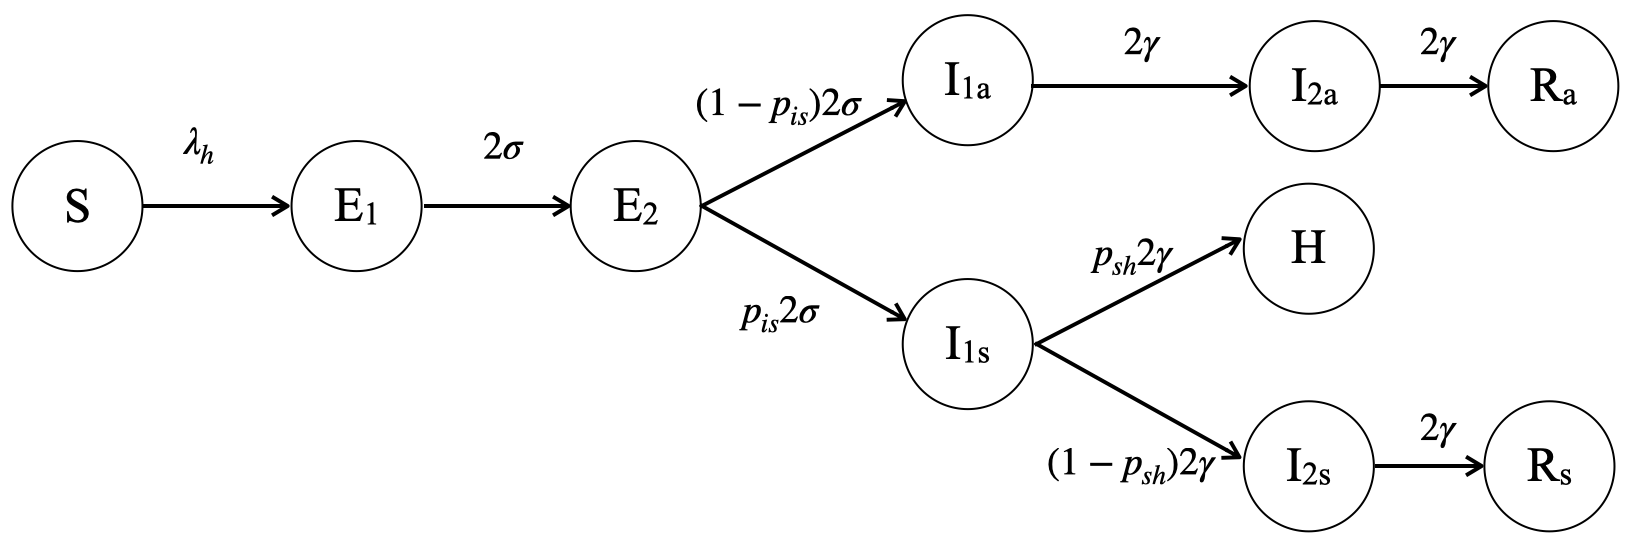
\includegraphics[scale=0.4]{Figs/SEEIIHR_markov_chain2.png}
	%		\vspace{-10mm}
	\caption{State diagram of the household SEEIIHR epidemic model at the individual level. Nodes show the possible states an individual may be in at a given time, edges show the transition probabilities between states. Transmission within household $h$ is given by $\lambda_h = \beta \frac{I_h}{k-1} + \alpha \frac{I_{tot}-I_h}{N-k}$.}
	\label{fig:SEEIIRH_model}
\end{figure}

\begin{table}[h!]
	\centering
	\caption{Transmission States of the Household SEEIIHR Epidemic Model}
	\begin{tabular}{p{0.1\linewidth}p{0.4\linewidth}}
%	\begin{tabular}[t]{l>{\raggedright\arraybackslash}p{0.5\linewidth}}
		%		\begin{tabular}[t]{l>{\raggedright\arraybackslash}p{0.7\linewidth}}
		\toprule
		State      & Definition \\
		\midrule
		$S$        & Susceptible \\
		$E_{1}$   & Exposed (stage 1) \\
		$E_{2}$   & Exposed (stage 2) \\
		$I_{1a}$   & Infectious asymptomatic (stage 1) \\
		$I_{2a}$   & Infectious asymptomatic (stage 2) \\
		$I_{1s}$   & Infectious symptomatic (stage 1) \\
		$I_{2s}$   & Infectious symptomatic (stage 2) \\
		$H$         & Hospitalised \\
		$R_a$     & Recovered (asymptomatic) \\
		$R_s$     & Recovered (symptomatic) \\
		\bottomrule
	\end{tabular}
	\label{tab: Transmission states}
\end{table}%

\begin{table}[h!]
	\centering
	\caption{Parameters of the SEEIIHR Household Transmission Model}
	\begin{tabular}{p{0.2\linewidth}p{0.5\linewidth}}
%	\begin{tabular}[t]{l>{\raggedright\arraybackslash}p{0.7\linewidth}}
		\toprule
		Parameter  & Definition \\
		\midrule
		$\alpha$    & Transmission rate within households \\
		$\beta$      & Transmission rate between households \\
		$\sigma$   & Transition rate from exposed to infected state \\
		$\gamma$ & Recovery rate \\
		$p_{is}$     & Probability an infected individual will be symptomatic \\
		$p_{sh}$    & Probability a symptomatic individual will be hospitalised \\
		$p_{ih} = p_{is}p_{sh}$  & Probability an infected individual will be hospitalised \\
		\bottomrule
	\end{tabular}
	\label{tab: Transmission parameters}
\end{table}

\begin{figure}[h!]
	\centering
	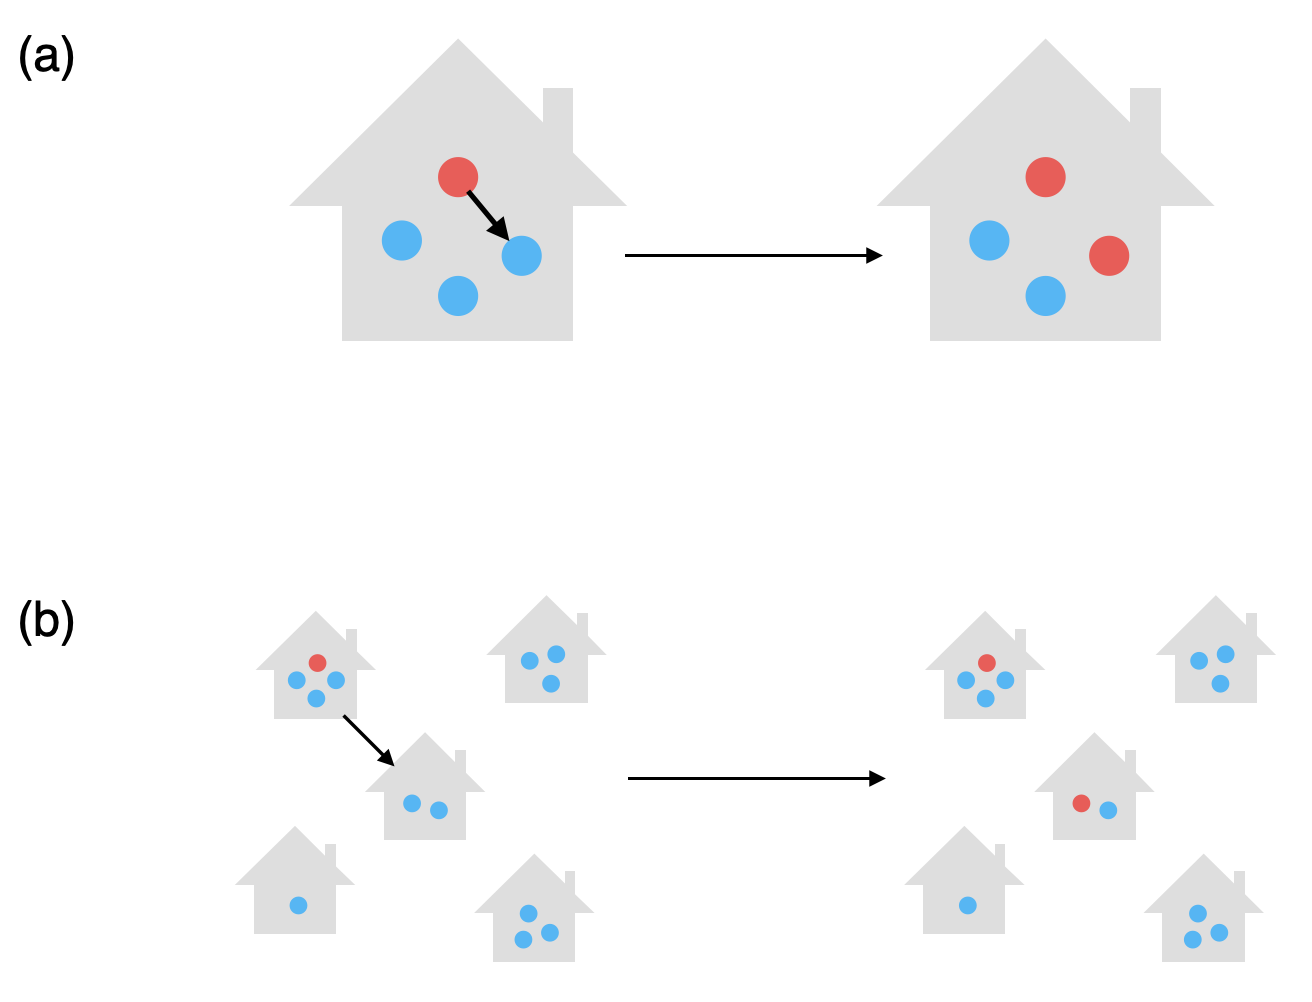
\includegraphics[scale=0.5]{Figs/hh_pop_model.png}
	\caption{A household model described by Ross \textit{et al.}. 2010 with (a) strong homogeneous mixing within households and (b) weaker mixing between households.}
	\label{fig:household_model}
\end{figure}

The observation model describes the capture of information about symptomatic and hospitalised individuals by three surveillance systems: FluTracking, FluCAN, and case notifications. First Few Hundred (FF100) were originally included in the MATRIX formulation, but are omitted here (discussed below). Each week, data collected by each surveillance system become available. In addition to true influenza cases, symptomatic and hospitalised cases of non-influenza ILI may also be detected by surveillance. Conversely, asymptomatic influenza cases are infectious and may transmit the disease to susceptible individuals, but remain invisible to surveillance.  \\
During the spread of the epidemic, new symptomatic and hospitalised cases occur at random times throughout the day. Denote the true number of new symptomatic cases in household $h$ at the end of week $t$ by $I_{st}^h$, and new hospitalised cases $H_t^h$, for $h=1,2,...,100$ and $t=1,2,...,14$. These are latent (unobserved) variables. The sum of these two quantities over all households gives the total number of new symptomatic cases ($I_{st}^p$) and new hospitalised cases ($H_t^p$) in the population at week $t$. Most of the time $I_{st}^p$ will be larger than $H_t^p$ since new hospitalised cases first had to become new symptomatic cases. However $I_{st}^p$ is not a subset of $H_t^p$, since a case may have become symptomatic one week and then hospitalised the week after. It is also possible that $H_t^p > I_{st}^p$, especially towards the end of the epidemic when new symptomatic cases are falling and those currently in the first symptomatic state are moving into the hospitalised state. These latent variables are the source from which the three surveillance systems capture their data. \\
A graphical representation of the observation model, showing the flow of new symptomatic and hospitalised cases from households into the various, possibly overlapping, surveillance systems is given by Figure~\ref{fig:Observation_model}.
Observation states are summarised in Table \ref{tab: Observation states}, and observation parameters are summarised in Table \ref{tab: Observation parameters}.
\begin{figure}[h!]
	\centering
	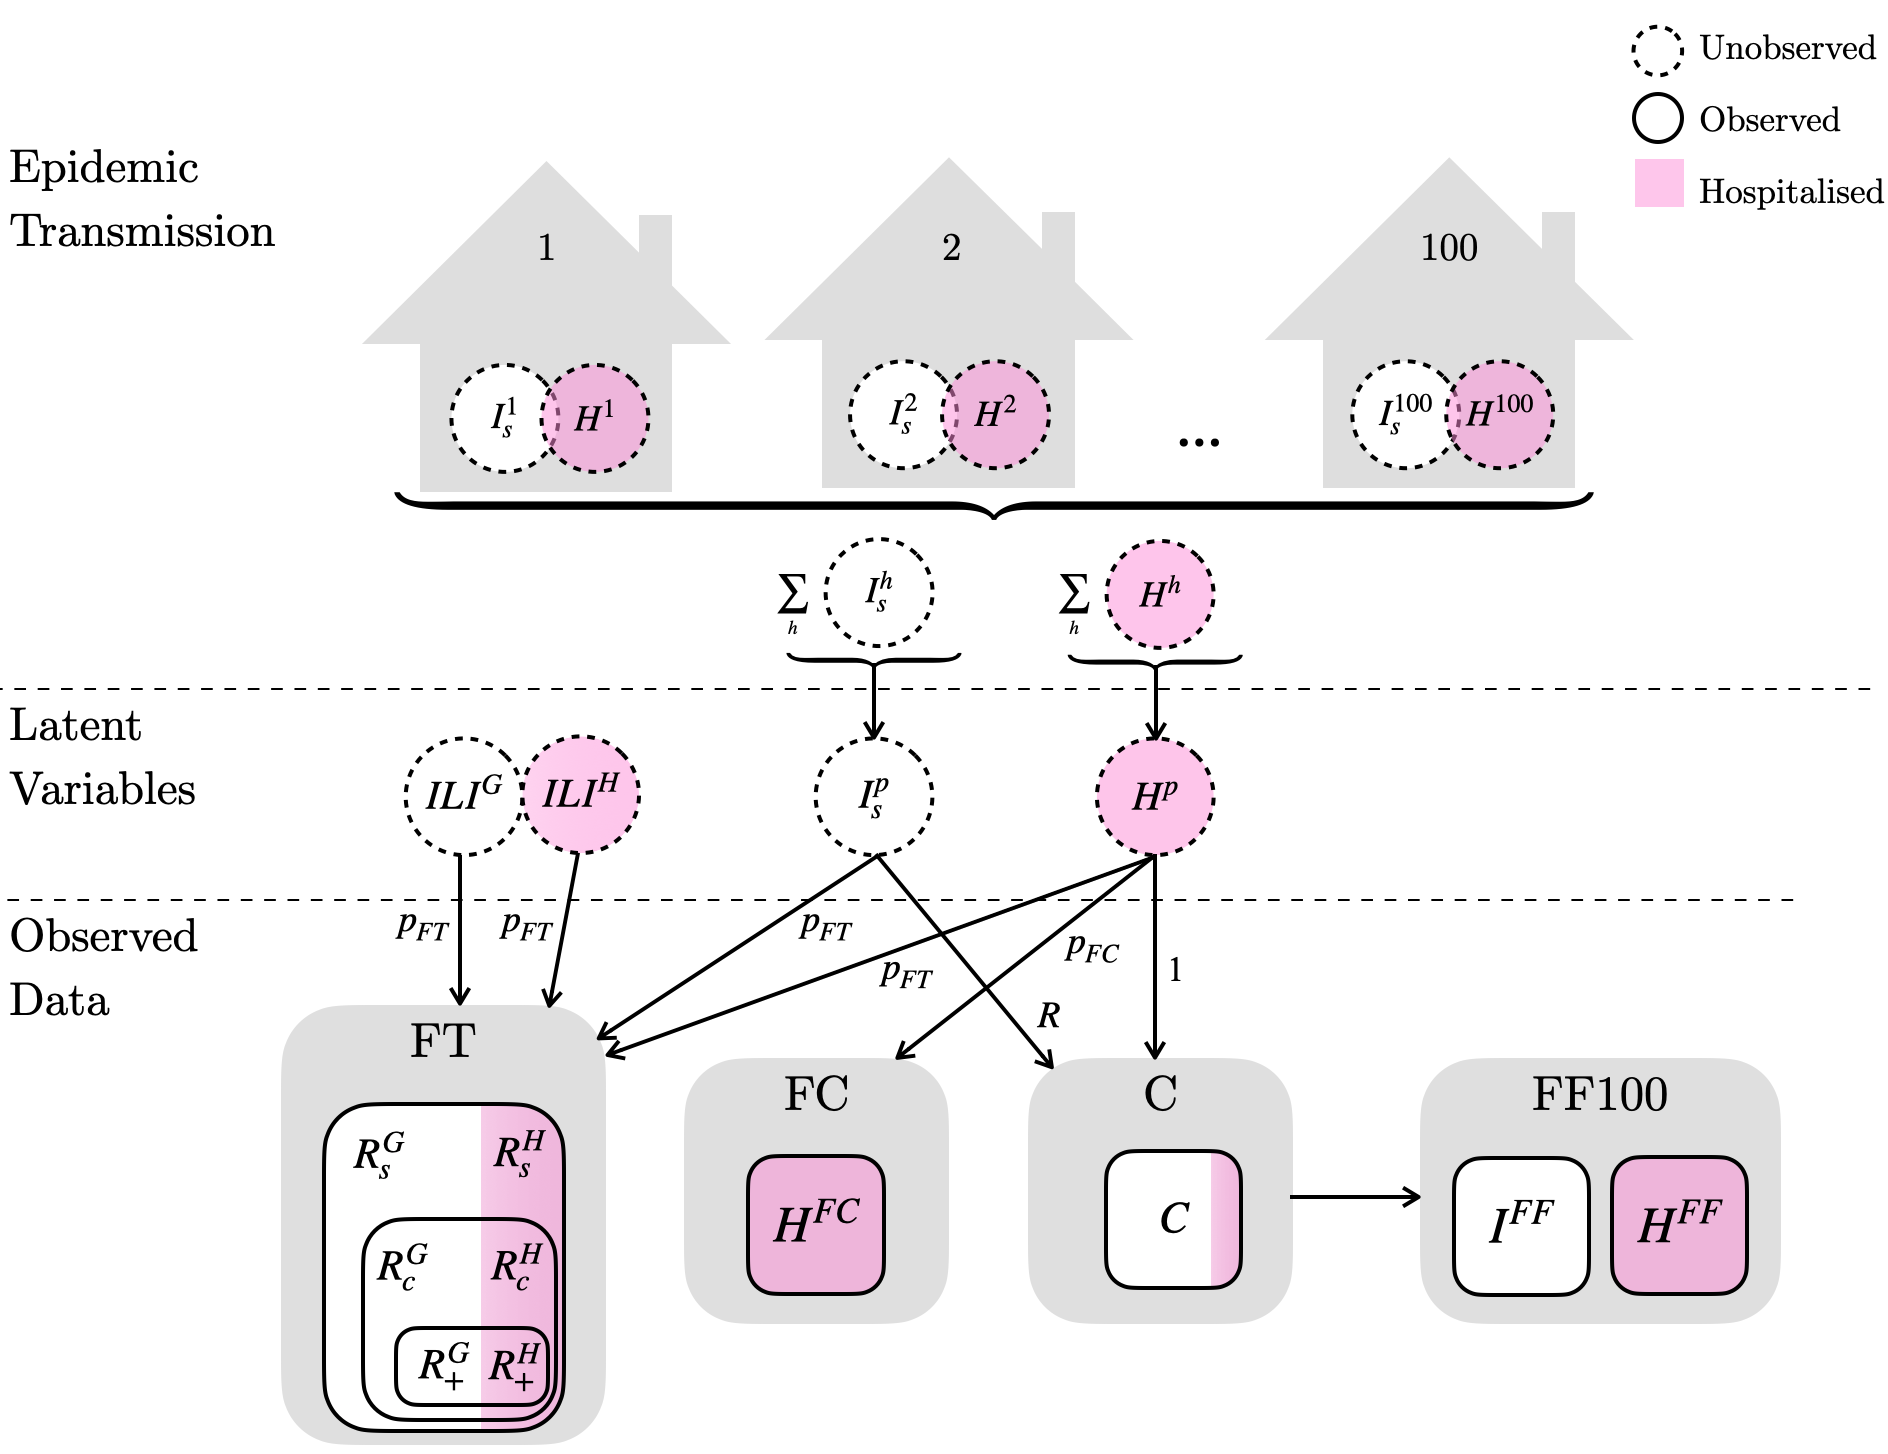
\includegraphics[scale=0.4]{Figs/Observation_model_diagram}
	%		\vspace{-10mm}
	\caption{Observation model showing the flow of unobserved symptomatic and hospitalised cases in the population ($I_s^p$, $H$) into the surveillance systems ($FT$, $FC$, $C$, $FF100$). Shapes in dashed lines indicate unobserved data, solid lines indicate observed data, pink shading indicates a proportion of hospitalised cases. Although regions representing data sets were not drawn to overlap as in a Venn diagram, there will almost certainly be cases common to at least two data sets e.g. case notifications also reported in FluTracking.}
	\label{fig:Observation_model}
\end{figure}

\subsection{FluTracking}
First consider the FluTracking surveillance system. A proportion $p_{FT}$ of the population is registered in FluTracking. Each week, a subset of all new symptomatic cases (influenza and ILI) report having symptoms with probability $p_{FT}$. Let $R_{st}^G$ denote the number of new cases reporting symptoms at week $t$, then $R_{st}^G \subset I_{st}^p + ILI_t^{G}$. A subset of those reporting symptoms also report having been tested for influenza at the GP ($R_{ct}^G$) with probability $p_{GPtest}$, i.e. $R_c^G \subset R_s^G$. Of the true influenza cases that report being tested, a subset ($R_{+t}^G$) report testing positive to influenza with probability $p_{+}$. Similarly for hospitalised case, $R_{+t}^H \subset R_{ct}^H \subset R_{st}^H \subset H_t^p + ILI_t^{H}$. FluTracking data therefore consist of six data sets $FT = \{R_s^G, R_c^G, R_+^G, R_s^H, R_c^H, R_+^H\}$.

\subsection{FluCAN}
FluCAN data consist of all laboratory-confirmed cases from hospitals that are part of FluCAN, which make up a proportion $p_{FC}$ of all hospitals in the city or state of interest. Therefore, the FluCAN data $H_t^{FC}$ represents a random sample of all new confirmed hospital cases at week $t$. Some of these cases are also registered with FluTracking, so FluCAN data are composed of cases that are unique to FluCAN ($H_t^{FC\setminus FT}$), and those that are detected by both FluCAN and FluTracking ($H_t^{FC\cap FT}$), i.e. $H_t^{FC} = H^{FC\setminus FT} + H_t^{FC\cap FT}$.

\subsection{Case Notification}
Finally, every laboratory-confirmed case of influenza, whether from a GP or hospital test, is reported as a case notification. Some of these cases may be unique to tests taken at the GP ($C_t^{GP^*}$) or hospital ($C_t^{H^*}$) at week $t$, however some may also be reported in FluTracking, which also may include FluCAN cases, and some may be recorded in FluCAN but not FluTracking. Therefore all case notification data at week $t$ are composed of six different subsets $C_t = C_t^{GP^*} + C_t^{H^*} + R_{+t}^H + H_t^{FC\setminus FT}$.\\ \\
A proportion of all case notifications could be enrolled into First Few Hundred (FF100) data. However, as including this data further complicates an observation model that already contains three surveillance systems, the FF100 data were not considered in this analysis. Future work could extend the scope of this observation model to include FF100 data. \\
\begin{table}[h!]
	\centering
	\caption{Observation Model Parameters}
	%	 	\begin{tabular}{l l}
%	\begin{tabular}[t]{l>{\raggedright\arraybackslash}p{0.7\linewidth}}
	\begin{tabular}{p{0.15\linewidth}p{0.7\linewidth}}
		\toprule
		Parameter  & Definition \\
		\midrule
		$I_s^h$, $I_s^p$	 & True number of symptomatic (not confirmed) cases in household $h$ / population (unobserved) \\
		$H_s^h$, $H_s^p$   & True number of laboratory-confirmed hospitalised cases in household $h$ / population (unobserved) \\
		$ILI^{G}$, $ILI^{H}$  & Number of symptomatic and hospitalised non-influenza ILI cases in population (unobserved) \\
		$p_{FT}$                 & Proportion of population enrolled in FluTracking \\
		$p_{FC}$                 & Proportion of hospital beds captured by FluCAN \\
		$R$                        & Probability a symptomatic case becomes case notification, i.e. $R = p_{GPtest}p_{+} = p_{Htest}p_{+}$ \\
		\bottomrule
	\end{tabular}
	\label{tab: Observation states}
\end{table}

\begin{table}[h!]
	\centering
	\caption{Observation Model Data}
	\begin{tabular}{p{0.15\linewidth}p{0.7\linewidth}}
		\toprule
		Data Set      & Description \\
		\midrule
		$R_{s}^G$, $R_{s}^H$   & Number of symptomatic cases reported in FluTracking \\
		$R_{c}^G$, $R_{c}^H$       & Number of cases tested for influenza reported in FluTracking \\
		$R_{+}^G$, $R_{+}^H$	    & Number of positive tests reported in FluTracking  \\
		$H^{FC}$	                 & Number of hospitalised cases recorded in FluCAN \\
		$C$		                        & Number of laboratory-confirmed case notifications \\
		\bottomrule
	\end{tabular}
	\label{tab: Observation parameters}
\end{table}	




\subsection{Model Implementation}

\subsubsection{Stochastic Simulation}
The household SEEIIHR epidemic model was simulated using Gillespie's $\tau$-leap algorithm, which approximates the direct method and was introduced briefly in Subsection \ref{subsec: stochastic simulation algorithm}. The two methods are very similar. The main difference is that instead of generating random time intervals between each transition event (see Figure \ref{fig:SEEIIRH_model}), the $\tau$-leap algorithm steps through time in intervals of $\tau$ and at each time step generates a random number of transitions for each transition event (e.g. $S\rightarrow E_1$). The $\tau$-leap algorithm is described in more detail here.\\
Let $\mathbf{X}=(S, E_1, E_2, I_{1a}, I_{2a}, I_{1s}, I_{2s}, H, R_a, R_s)$ denote the current state of the system. For the SEEIIHR model there are 9 transition events, $S \rightarrow E_1$ etc. Let $Z_{i}$ denote the $i$th transition event, $i=1,2,...,9$, i.e.
\begin{align} \notag
	Z_1 &= \{S \rightarrow E_1 \} \\ \notag
	Z_2 &= \{E_1 \rightarrow E_2 \} \\ \notag
	Z_3 &= \{E_2 \rightarrow I_{1a} \} \\ \notag
	Z_4 &= \{I_{1a} \rightarrow I_{2a} \} \\ \notag
	Z_5 &= \{E_2 \rightarrow I_{1s} \} \\ \notag
	Z_6 &= \{I_{1s} \rightarrow I_{2s} \} \\ \notag
	Z_7 &= \{I_{1s} \rightarrow H \} \\ \notag
	Z_8 &= \{I_{2a} \rightarrow R_a \} \\ \notag
	Z_9 &= \{I_{2s} \rightarrow R_s \}
\end{align}
The so-called stoichiometric matrix $\mathbf{v}$ determines the effect of each event type on the number of individuals in each state and has the dimensions (\#events $\times$ \#states). For example, the first row in $\mathbf{v}_1 = (-1, +1, 0, 0, 0, 0, 0, 0, 0, 0)$ corresponds to the first event $S \rightarrow E_1$ such that $\mathbf{X} + \mathbf{v}_{1} = (S-1, E_1+1, E_2, I_{1a}, I_{2a}, I_{1s}, I_{2s}, H, R_a, R_s)$.
Transition rates are determined by the transition probabilities between events (see Figure \ref{fig:SEEIIRH_model})
\begin{align} \notag
	r_1 &= \frac{\alpha I_{tot}+\beta I_h}{N-1} S \\ \notag
	r_2 &= 2\sigma E_1 \\ \notag
	r_3 &= 2\sigma (1 - p_{is}) E_2 \\ \notag
	r_4 &= 2\gamma I_{1a} \\ \notag
	r_5 &= 2\sigma p_{is} E_2 \\ \notag
	r_6 &= 2\gamma (1-p_{sh}) I_{1s} \\ \notag
	r_7 &= 2\gamma p_{sh} I_{1s}  \\ \notag
	r_8 &= 2\gamma I_{1a}  \\ \notag
	r_9 &= 2\gamma I_{1s}
\end{align}
Gillespie's $\tau$-leaping algorithm is implemented by the following steps:

\begin{enumerate}
	\item \textbf{Initialise}. Set initial state $\mathbf{X}_0$,  compute transition rates $r_j$ for events $Z_j$, $j=1,2,...,m$, and choose time interval $\tau$.
	
	\item \textbf{Generate Transition Events}. At time $t$:
	\begin{enumerate}[]
		\item For each event type $j$, generate number of events $K_j \sim$ Poi($r_j\tau)$.
		\item Update all states $\mathbf{X}(t+\tau) = \mathbf{X}(t) + \sum_j K_j \mathbf{v}_{ij}$, where $v_{ij}$ is the change on state $i$ due to event $j$.
	\end{enumerate}

	\item \textbf{Iterate}. Set $t \leftarrow t + \tau$. If $t=T$ stop, else go back to step 2.
	
\end{enumerate}
\noindent States were initialised using three infected individuals randomly distributed over three separate households. The rest of the population was susceptible, i.e. $S=10^5-3$  with the number of individuals in all remaining states set to zero.\\
The $\tau$-leaping algorithm was used first to generate the `true' epidemic process from which the data were collected (Figure \ref{fig: SEEIIHR trajectories}) for the parameter estimation process.
\begin{figure}[h!]
	\centering
	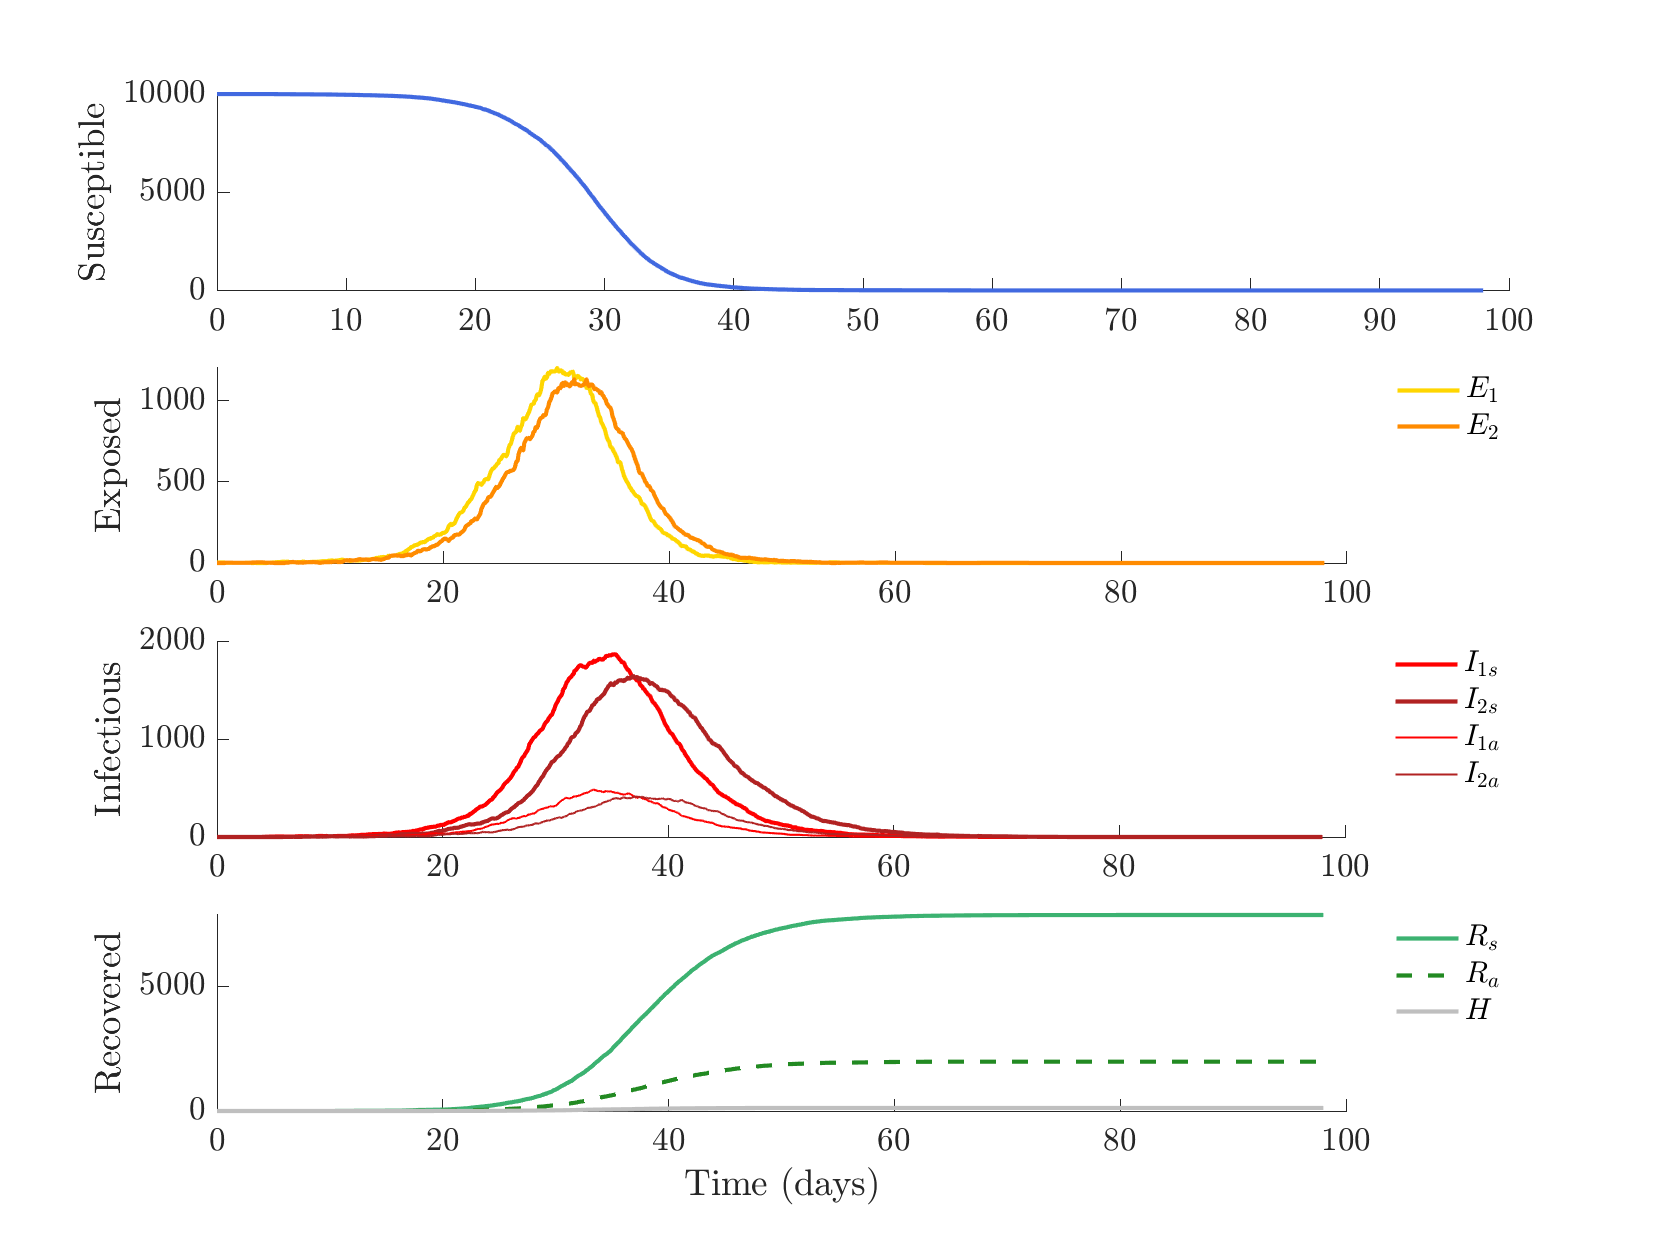
\includegraphics[scale=0.5]{Figs/SEEIIHRR_trajectories.png}
	%		\vspace{-10mm}
	\caption{Realisation of the stochastic household SEEIIHR epidemic model that served as the `true' epidemic from which data were collected. Plots show the number of individuals in each state over time: susceptible (blue), exposed (yellow colours), infectious (red colours), hospitalised (grey) and recovered (green colours). Dashed lines indicate asymptomatic cases.}
	\label{fig: SEEIIHR trajectories}
\end{figure}

\subsection{Generation of Data}
The MATLAB implementation of the SEEIIHR epidemic model generated a `true' unobserved number of new symptomatic ($I_s^p$) and hospitalised ($H^p$) cases in the population over time. These quantities were stored at weekly intervals and were used to generate the data that would in reality be collected by the surveillance systems described in Section \ref{sec: observation model}. This process of generating synthetic data for each surveillance system is described here. In the notation below the time subscript $t$ is dropped for convenience.

\subsubsection{FluTracking}
Recall FluTracking data are composed of six data sets depending on what individuals report: $FT = \{R_{s}^G,R_{c}^G,R_{+}^G,R_{s}^H,R_{c}^H,R_{+}^H\}$. These include cases of influenza, but also new symptomatic ($ILI^{Gnf}$ ) and hospitalised cases ($ILI^{Hnf}$) due to a non-influenza ILI. The structure of these data sets are now considered in more detail.\\
The number of individuals who report becoming symptomatic but not hospitalised ($R_{s}^G$) is made up of those with influenza ($R_{s}^{Gf}$) and those with an ILI ($R_{s}^{Gnf}$), i.e.
\begin{align} \notag
R_{s}^{G} &= R_{s}^{Gf} + R_{s}^{Gnf},
\end{align}
where $R_{s}^{Gf}$ and $R_{s}^{Gnf}$ were drawn from the binomial distribution using the binornd(n,p) function in MATLAB:
\begin{align} \notag
R_{s}^{Gf} &\sim binom(I_{s}^p,p_{FT}), \\ \notag
R_{s}^{Gnf} &\sim binom(ILI^{Gnf},p_{FT}).
\end{align}
The number of participants who reported going to the GP and being tested is composed of those with influenza ($R_{c}^{Gf}$) and those with an ILI ($R_{c}^{Gnf}$)
\begin{align} \notag
	R_{c}^{G} &= R_{c}^{Gf} + R_{c}^{Gnf},
\end{align}
where $R_{c}^{Gf}$ and $R_{c}^{Gnf}$ are binomial random variables
\begin{align} \notag
	R_{c}^{Gf} &\sim binom(R_{s}^{Gf},p_{GPtest}), \\ \notag
	R_{c}^{Gnf} &\sim binom(R_{s}^{Gnf},p_{GPtest}).
\end{align}
Of the participants who were symptomatic, who went to the GP and were tested, the number who test positive $R_{+}^{Gf}$ is a binomially distributed random variable that depends only on the number with influenza ($R_{c}^{Gf}$) and the sensitivity of the test ($p_+$)
\begin{align} \notag
	R_+^G &\sim binom(R_{c}^{Gf},p_+).
\end{align}
Similarly the hospitalised cases $R_{s}^H$ is the sum of those with influenza ($R_{s}^{Hf}$) and those without ($R_{s}^{Hnf}$)
\begin{align} \notag
R_{s}^{H} = R_{s}^{Hf} + R_{s}^{Hnf},
\end{align} 
where 
\begin{align} \notag
R_{s}^{Hf} &\sim binom(H_{s}^p,p_{FT}), \\ \notag
R_{s}^{Hnf} &\sim binom(ILI^{Hnf},p_{FT}).
\end{align}
Again, those who reported going to hospital and being tested is made up of those with influenza and those with an ILI,
\begin{align} \notag
R_{c}^{H} &= R_{c}^{Hf} + R_{c}^{Hnf},
\end{align}
where
\begin{align} \notag
R_{c}^{Hf} &\sim binom(R_{s}^{Hf},p_{Htest}), \\ \notag
R_{c}^{Hnf} &\sim binom(R_{s}^{Hnf},p_{Htest}).
\end{align}
Finally, the number who report testing positive depends only on the number with influenza who get tested and the sensitivity of the test
\begin{align} \notag
	R_+^H &\sim binom(R_{c}^{Hf},p_+).
\end{align}

\subsubsection{FluCAN}
%$H^{FC}_t = P^{FC} \times H_{weekly}$
FluCAN data only capture a portion of hospitalised laboratory-confirmed cases in the population, some of which may have been reported in FluTracking ($R_{+}^H$). So the number of individuals in FluCAN is made up of those in both FluCAN and FluTracking ($H^{FC\cap FT}$), and those only in FluCAN ($H^{FC \setminus FT}$). That is
\begin{align} \notag
H^{FC} &= H^{FC \setminus FT} + H^{FC \cap FT}
\end{align}
where $H^{FC \cap FT}$ depends on the number reporting a positive hospital test in FluTracking ($R_{+}^H$) and the proportion of those being from FluCAN hospitals ($p_{FC}$), and $H^{FC \setminus FT}$ depends on the unobserved number of new hospitalised cases minus those reporting positive hospital tests in FluTracking, and the compound probability of being in FluCAN, being tested, and the test being positive ($p_{FC}p_{Htest}p_+$), i.e.
\begin{align} \notag
H^{FC \cap FT} &\sim binom(R_{+}^H ,p_{FC}), \\ \notag
H^{FC \setminus FT} &\sim binom(H^P - R_{+}^H, p_{FC}p_{Htest}p_+).
\end{align}

\subsubsection{Case notifications}
New case notifications each week ($C$) are the sum of all positive cases (GP and hospital cases), some of which may be included in FluTracking or FluCAN. Therefore, case notifications are conditional on both the latent data ($I_s^p$, $H^p$), FluTracking, and FluCAN.
New weekly case notifications that are unique to GP tests ($C^{GP^*}$) are binomially distributed and depend on the number of new symptomatic cases minus positive cases reported in FluTracking and the probability of being tested at the GP and testing positive. Unique hospital cases ($C^{H^*}$) depend on the number of new hospital cases minus positive cases reported in FluTracking and FluCAN cases, and the probability of being tested in hospital and testing positive, i.e.
\begin{align} \notag
C^{GP^*} &\sim binom(I^p-R_{+}^G, p_{GPtest}p_{+}), \\ \notag
C^{H^*} &\sim binom(H^p-R_{+}^H-H^{FC \setminus FT}, p_{Htest}p_{+}).
\end{align}
The total number of new cases notifications each week is therefore
\begin{align} \notag
	C &= C^{GP^*} + C^{H^*} + R_{+}^{G} + R_{+}^H + H^{FC \setminus FT}.
\end{align}
\noindent A time series of the latent variables ($I_s^p$, $H^p$), and the surveillance data produced by the simulation of the household SEEIIHR model, are shown in Figure \ref{fig: synthetic data}.
%FluCAN and case notification data are presented as the sum of their unobserved components.

%\newpage
\begin{figure}[h!]
	%	\centering
	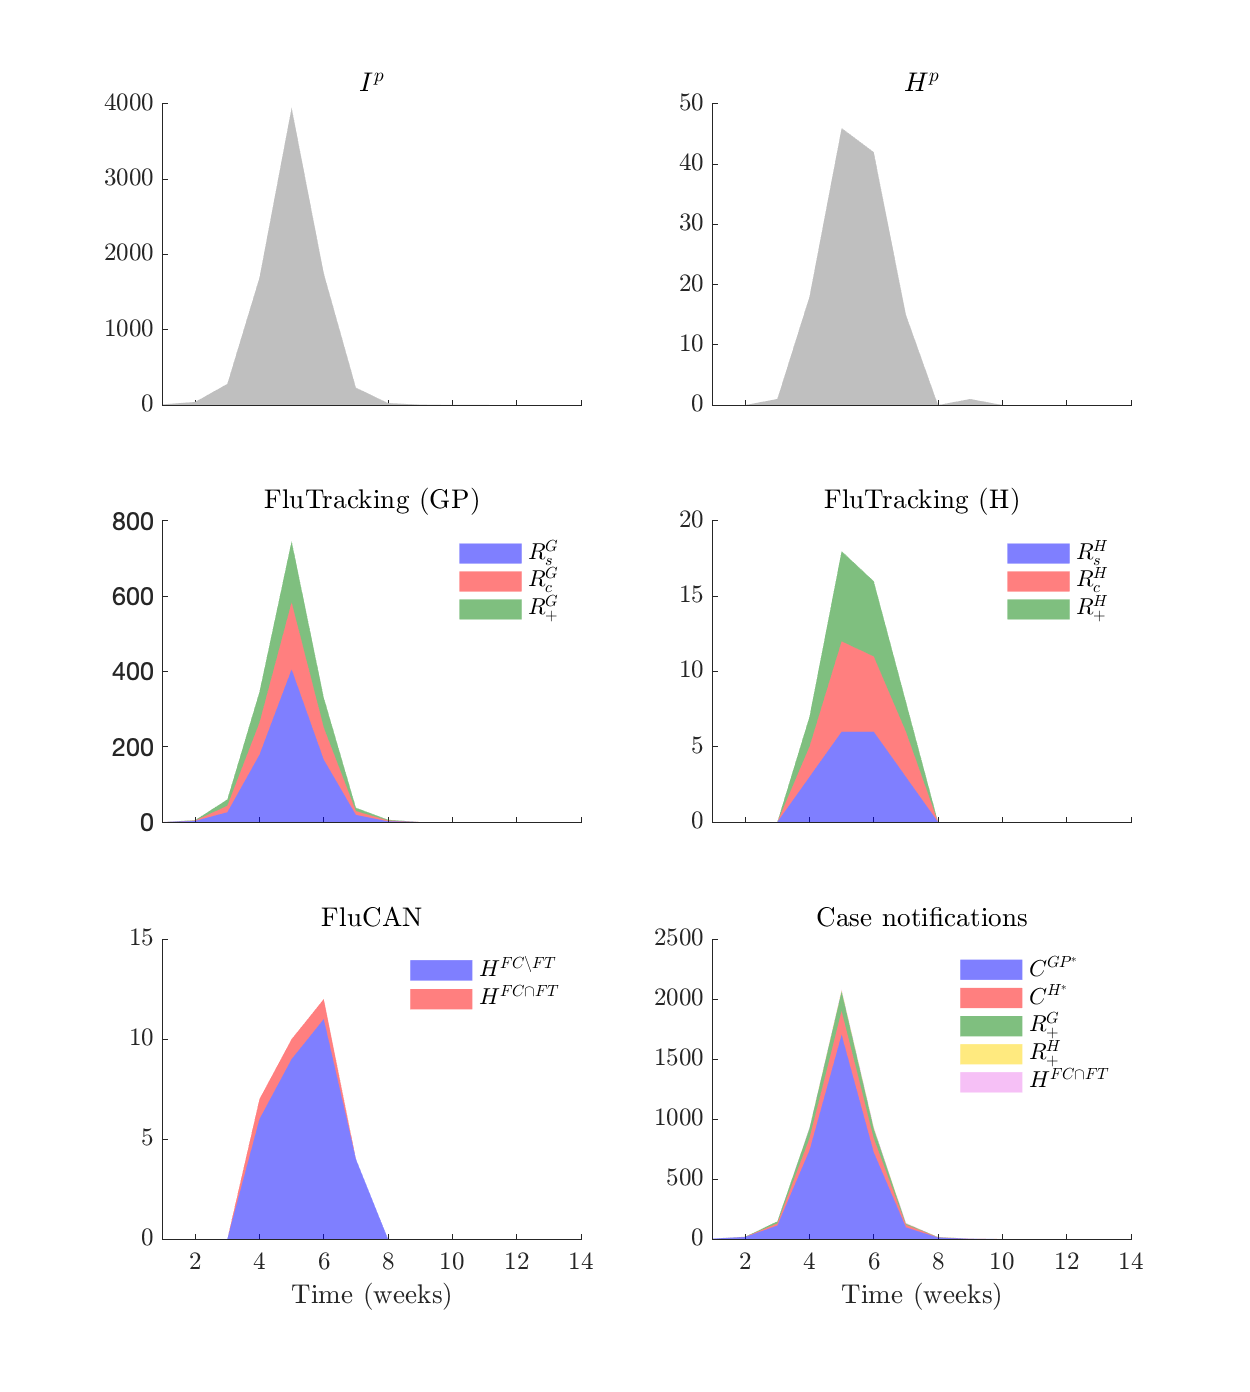
\includegraphics[scale=0.75]{Figs/allDataPlot.png}
	%		\vspace{-10mm}
	\caption{Data generated over 14 weeks by the SEEIIHR epidemic model including the unobserved true processes $I^p$ and $H^p$. The observed data for FluTracking, FluCAN, and case notifications are composed of unobserved variables (dashed lines) eg. FluCAN's $H^{FC\cap FT}$ and $H^{FC\setminus FT}$.}
	\label{fig: synthetic data}
\end{figure}


\subsection{Bayesian Inference}
Given weekly surveillance data $FT$, $FC$ and $C$, we want to estimate the transmission model parameters $\theta = (\alpha, \beta, \sigma, \gamma, p_{is}, p_{sh})$. For the Bayesian inference it is necessary to compute the posterior distribution of the transmission parameters given the data, i.e.
\begin{align} \notag
P(\theta | FT, FC, C) &\propto P(FT, FC, C | \theta) P(\theta)
\end{align}
where $P(FT, FC, C|\theta)$ is the likelihood of the data and $P(\theta)$ is the joint prior distribution of the parameters. In the following sections, the likelihood of the data and the joint prior are constructed. However, computational constraints mean that computing the log of the likelihood and joint prior is preferred. The Metropolis-Hastings algorithm in the context of the multidata household SEEIIHR epidemic model is described in more detail, including a modification of the general algorithm to the log-scale and the proposal distribution for generating new samples. Finally, this chapter ends with a summary of the overall process from generating the observed data to inferring the model parameters.

\subsubsection{Likelihood}
The likelihood of the data given the model parameters $L = P(FT, FC, C | \theta)$ can be constructed using the structure presented in Section \ref{subsec: lit rev likelihood}. Here the latent (unobserved) data are the number of new infections $I^p$ and the number of new hospitalised cases $H^p$ each week. By marginalising over, and then conditioning on, these latent data the likelihood $L$ can be expressed
\begin{align} \label{Param est: likelihood as expectation} \notag
L &= P(FT, FC, C | \theta) \\ \notag
&= \sum_{I^p, H^p} P(FT, FC, C, I^P, H^P, | \theta) \\
&= \sum_{I^p, H^p} P(FT, FC, C| I^P, H^P, \theta) P( I^P, H^P |\theta).
\end{align}
Recall that for a discrete random variable $X$ that takes the values $x_1, x_2,..., x_n$ with probabilities $p_1, p_2,..., x_n$ the expected value of $X$ is $\mathbb{E}[X] = \sum_{i=1}^n x_i p_i$. It follows that the likelihood can be expressed as the expected value of $P(FT, FC, C| I^P, H^P, \theta) $
\begin{align}
P(FT, FC, C | \theta) &= \mathbb{E}[ P(FT, FC, C| I^P, H^P, \theta) ].
\end{align}
This expectation can be approximated using the pseudo-marginal estimate, i.e. by calculating the sample mean over $M$ realisations of $I^p$ and $H^p$ generated from the multi-data household SEEIIHR epidemic model described in Section \ref{sec: transmission model}
\begin{align} \notag \label{eqn: posterior as average}
	L &= \mathbb{E}[ P(FT, FC, C| I^P, H^P, \theta) ]\\
	&\approx \frac{1}{M} \sum_{m=1}^{M} P(FT, FC, C| I_m^P, H_m^P, \theta).
\end{align}
The implementation of this process is outlined in Algorithm \ref{alg: compute likelihood}.
The goal of this section is to derive an expression for $P(FT, FC, C| I^P, H^P, \theta)$. To do this, in the following subsections $P(FT, FC, C| I^P, H^P, \theta)$ is expressed in terms of its component data sets. Then each component is derived in closed form. Finally these components are then brought together into a single closed form expression. \\ \\
\begin{algorithm}[H]
	\caption{Approximate the likelihood using the pseudo-marginal estimate} \label{alg: compute likelihood}
	\SetAlgoLined
%		\KwResult{Write here the result }
	Given the data set $FT$, $FC$, and $C$, and sufficiently large $M$\;
	\For{$m=1:M$}{
		Simulate the stochastic household SEEIIHR model in order to generate one realisation of $I_m^p$ and $H_m^p$ \;
		Calculate and store $P(FT, FC, C | I_m^p, H_m^p, \theta)$ \;
	}
	Average $P(FT, FC, C | I_m^p, H_m^p, \theta)$ over $M$ to obtain an unbiased estimate of the likelihood $P(FT, FC, C | \theta) = \frac{1}{M} \sum_{m=1}^{M} P(FT, FC, C | I_m^p, H_m^p, \theta)$
\end{algorithm}

Recall from Section \ref{sec: observation model} that FluTracking data consists of six data sets \{$R_s^G,R_c^G, R_+^G, R_s^H, R_c^H, R_+^H$\}, FluCAN consists of $H^{FC}$, and case notification data are denoted by $C$, then
\begin{align} \notag
	P(FT,FC,C | I^p, H^p, \theta) &= P(R_s^G,R_c^G, R_+^G, R_s^H, R_c^H, R_+^H, H^{FC},C | I^p, H^p, \theta).
\end{align}
This is further rearranged using the independence of the three surveillance systems and the dependencies on latent variables and observed data (Figure~\ref{fig:DAG}). It is possible to write
\begin{align} \notag
	P(R_s^G,R_c^G, R_+^G, R_s^H, R_c^H, R_+^H, H^{FC},C | I^p, H^p, \theta) &= P(R_s^G,R_c^G, R_+^G, R_s^H, R_c^H, R_+^H | I^p, H^p, \theta)\\ \notag
	&\times P(H^{FC}| H^p, R_+^H, \theta) \\
	&\times P(C | I^p, H^p, R_+^G, R_+^H, H^{FC}, \theta).
\end{align}

\begin{figure}[h!]
	\centering
	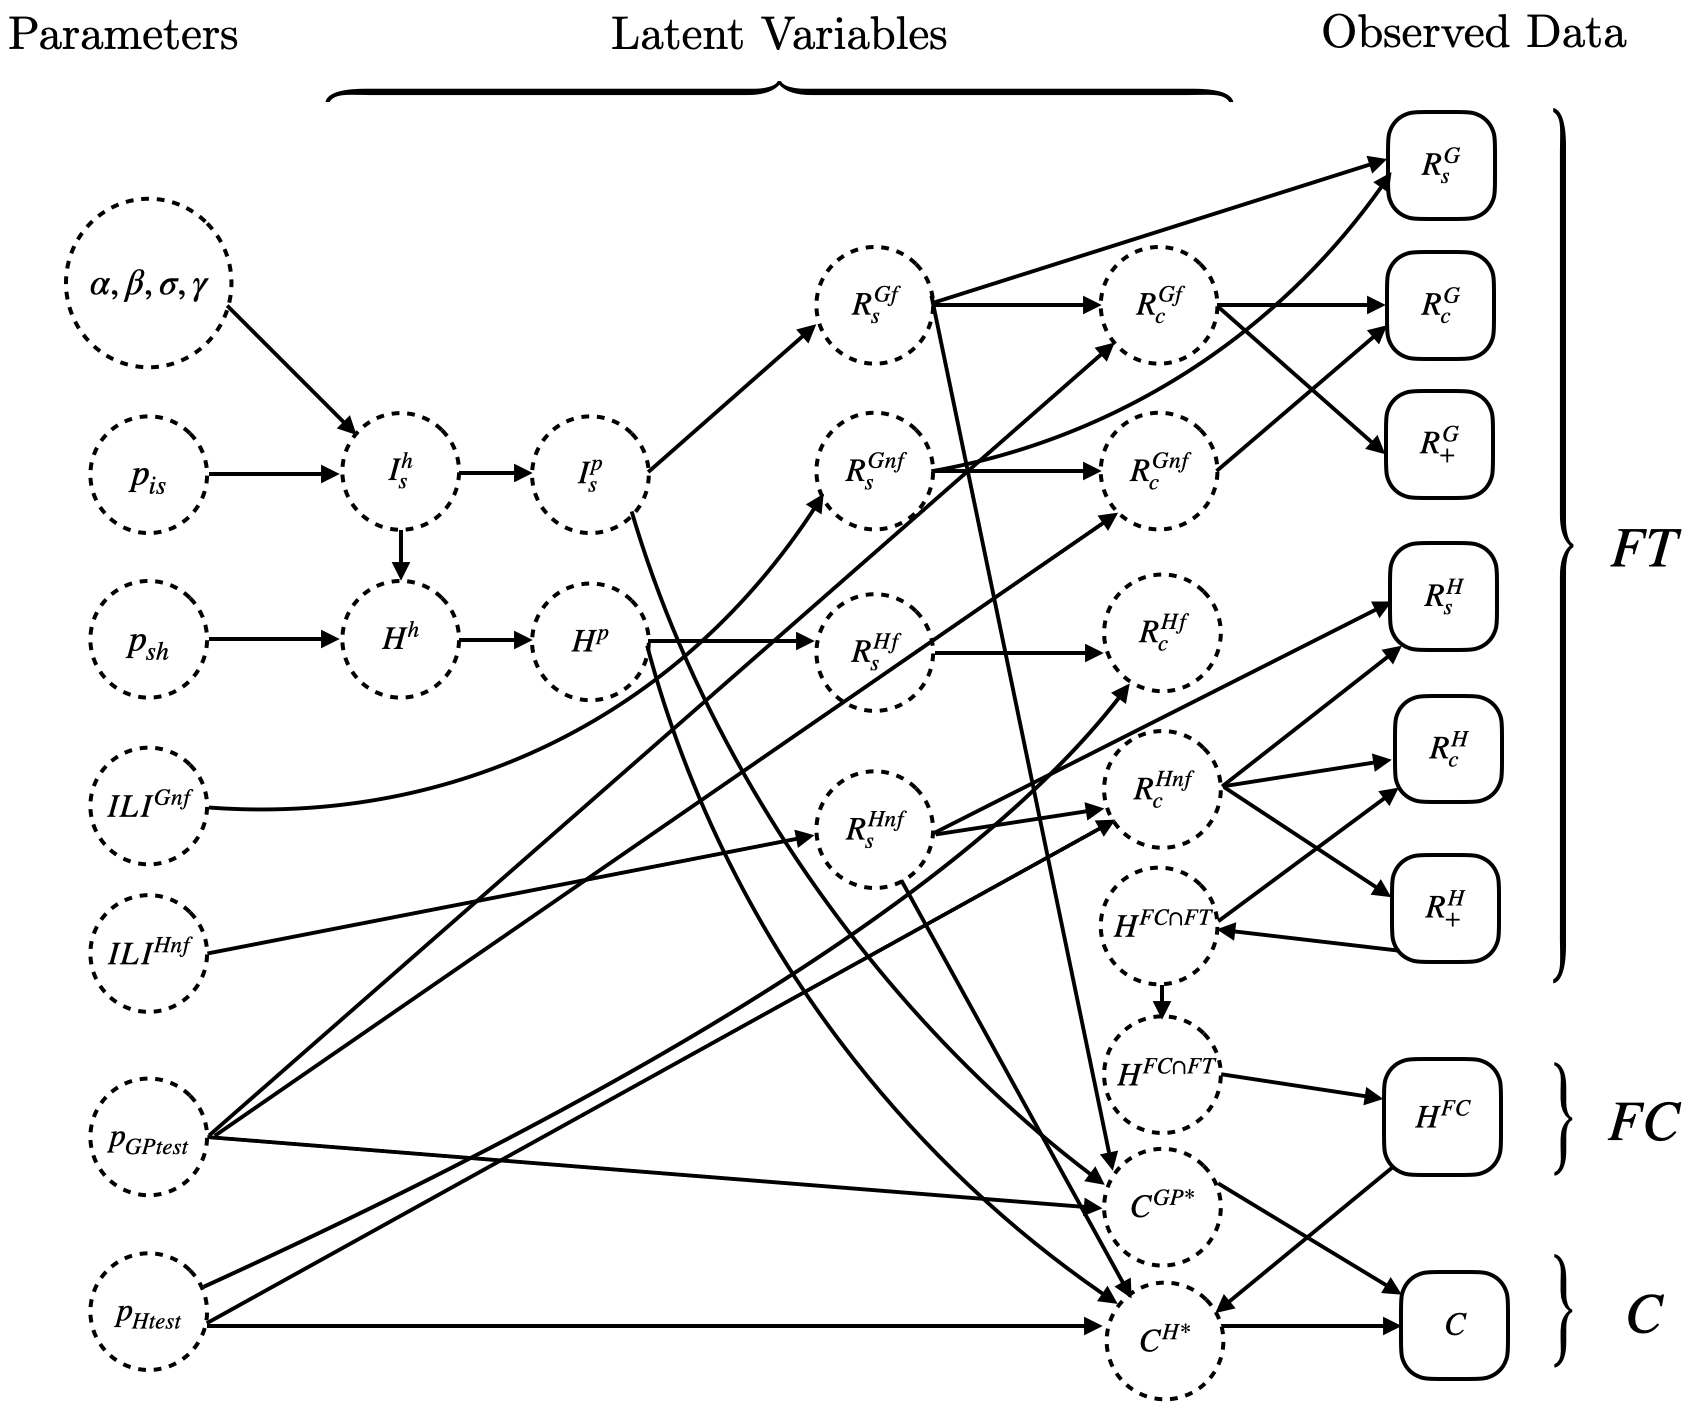
\includegraphics[scale=0.45]{Figs/DAG_noFF100.png}
	%		\vspace{-10mm}
	\caption{Conditional dependence of surveillance systems FluTracking ($FT$), FluCAN ($FC$), and case notifications ($C$) on transmission parameters $\{ \alpha, \beta, \gamma, \sigma, p_{is}, p_{sh} \}$, non-influenza ILI cases $ILI^{Gnf}, ILI^{Hnf}$ and testing parameters $p_{GPtest}, p_{Htest}$.}
	\label{fig:DAG}
\end{figure}

\noindent Observe that each data set $R_s^G, H^{FC}$ etc. is composed of sub-sets of data that are unobserved. For example, the number of people who report symptoms in FluTracking is composed of those with influenza and those with an ILI, i.e. $R_s^G = R_s^{Gf} + R_s^{Gnf}$. The law of total probability provides a way to compute probabilities in this case. For illustration, consider a random variable ($X$) that is composed of two unobserved independent random variables, $X=A+B$. Suppose the probability densities of $A$ and $B$ are known. It is possible to evaluate the probability $P(X=x)$ using the law of total probability and marginalising over the possible values of $A$ :
\begin{align} \label{total prob} \notag
	P(X=x) &= \sum_{a} P(X=x, A=a) &\text{(law of total probability)}\\
	&= \sum_{a} P(B=x-a|A=a) P(A=a) & \text{(marginalise over A)}.
\end{align}
This principle is repeated in the derivations of the components of the likelihood for each source of data below.

%\newpage
\subsection{FluTracking}
Here the FluTracking component of the likelihood $P(R_s^G,R_c^G, R_+^G, R_s^H, R_c^H, R_+^H | I^p, H^p, \theta)$ is derived. The probabilities for the non-hospitalised and hospitalised data may be considered independent, hence
\begin{align} \notag
	P(R_s^G,R_c^G, R_+^G, R_s^H, R_c^H, R_+^H | I^p, H^p, \theta) &= P(R_s^G,R_c^G, R_+^G | I^p, \theta ) \\ \label{eq: P(FT) joint}
	&\times P(R_s^H, R_c^H, R_+^H | H^p, \theta)	
\end{align}
First consider the non-hospitalised FluTracking data $\{R_s^G,R_c^G, R_+^G\}$. Recall that $R_s^G$ is the number of people who report symptoms, $R_c^G$ is the number of people who report being tested at the GP, and $R_+^G$ is the number who report testing positive from a GP test. The data sets $R_s^G$ and $R_c^G$ are each composed of cases who actually have influenza and those who have an ILI, i.e. $R_{s}^{G} = R_{s}^{Gf} + R_{s}^{Gnf}$, and $R_{c}^{G} = R_{c}^{Gf} + R_{c}^{Gnf}$ which follow the binomial distributions
\begin{align} \label{P(R_s^G)}
R_{s}^{Gf} | I^{p} &\sim binom(I^{p}, p_{FT}) \\ \label{P(R_c^G)}
R_{c}^{Gf} | R_{s}^{Gf} &\sim binom(R_{s}^{Gf}, P_{GPtest}) \\ \label{P(R_+^G)}
R_+^G | R_{c}^{Gf} &\sim binom(R_{c}^{Gf}, p_+) \\ \label{P(R_s^Gnf)}
R_s^{Gnf} | ILI^{Gnf} &\sim binom(ILI^{Gnf},p_{FT}) \\ \label{P(R_c^Gnf)}
R_c^{Gnf} | R_s^{Gnf} &\sim binom(R_{s}^{Gf},p_{GPtest})
\end{align}
It is possible to construct the likelihood for these data using the law of total probability (Equation \ref{total prob}) and marginalising over the true number of influenza cases who reported having symptoms $R_s^{Gf}$ and being tested $R_c^{Gf}$. The influenza cases who reported symptoms must be greater than the number who reported being tested and less than the total number who reported symptoms, $R_c^{Gf} \leq R_s^{Gf} \leq R_s^{G}$. Similarly, the number of influenza cases who report being tested $R_c^{Gf}$ must be greater than the number who report testing positive $R_+^{G}$ and less than the total number who reported being tested, $R_+^{G} \leq R_c^{Gf} \leq R_c^{G}$, so that:
\begin{align} \notag
%	&= \sum_{R_{c}^{Gf}=R_+^{G}}^{R_c^{G}} \sum_{R_{s}^{Gf}=R_{c}^{Gf}}^{R_{s}^{G}} P(R_s^G, R_{c}^{G}, R_{+}^{G}, R_{c}^{Gf}, R_{s}^{Gf} | I^p, \theta) \\ \notag
	P(R_{s}^{G}, R_{c}^{G}, R_+^G | I^p, \theta) 
	&= \sum_{R_{c}^{Gf}=R_+^{G}}^{R_c^{G}} \sum_{R_{s}^{Gf}=R_{c}^{Gf}}^{R_{s}^{G}} P(R_s^G, R_{c}^{G}, R_{+}^{G} | R_{c}^{Gf}, R_{s}^{Gf}, I^p, \theta) P(R_{c}^{Gf}, R_{s}^{Gf}| I^p, \theta)\\ \notag
	&= \sum_{R_{c}^{Gf}=R_+^{G}}^{R_c^{G}} \sum_{R_{s}^{Gf}=R_{c}^{Gf}}^{R_{s}^{G}} P(R_s^G-R_{s}^{Gf}, R_{c}^{G}-R_{c}^{Gf}, R_{+}^{G} | R_{c}^{Gf}, R_{s}^{Gf}, I^p, \theta) \label{eq: P(FT)} \\
	&\times P(R_{c}^{Gf}, R_{s}^{Gf}| I^p, \theta)\\ \notag
	&= \sum_{R_{c}^{Gf}=R_+^{G}}^{R_c^{G}} \sum_{R_{s}^{Gf}=R_{c}^{Gf}}^{R_{s}^{G}} P(R_+^G | R_{c}^{Gf}, p_+) P(R_c^{G} -R_c^{Gf}| R_{c}^{Gf}, p_{GPtest}) \\ 
	&\times P(R_{c}^{Gf} | R_{s}^{Gf}, \theta)	\times P(R_{s}^{G} -R_{s}^{Gf} | R_{s}^{Gf}, I^p, \theta) P(R_{s}^{Gf} | I^p),
\end{align}
having used the dependencies shown in Figure \ref{fig:DAG} to simplify Equation (\ref{eq: P(FT)}).
These probabilities follow binomial distributions defined by Equations (\ref{P(R_s^G)})-(\ref{P(R_c^Gnf)}) and can be expressed in closed form:
\begin{align}
P(R_{s}^{Gf} | I^p) &= \binom{I^p}{R_{s}^{Gf}} p_{FT}^{R_{s}^{Gf}}(1-p_{FT})^{I^p-R_{s}^{Gf}} \\
P(R_{c}^{Gf} | R_{s}^{Gf}) &= \binom{R_{s}^{Gf}}{R_{c}^{Gf}} 
p_{GPtest}^{R_{c}^{Gf}}(1-p_{GPtest})^{R_{s}^{Gf}-R_{c}^{Gf}} \\
P(R_+^G | R_{c}^{Gf}) &= \binom{R_{c}^{Gf}}{R_{+}^G}p_+^{R_{+}^G}(1-p_+)^{R_{c}^{Gf}-R_{+}^G} \\
P(R_{s}^{G}-R_{s}^{Gf} | ILI^{Gnf}) &= \binom{ILI^{Gnf}}{R_{s}^{G}-R_{s}^{Gf}} p_{FT}^{R_{s}^{G}-R_{s}^{Gf}}(1-p_{FT})^{ILI^{Gnf}-R_{s}^{G}+R_{s}^{Gf}} \\
P(R_{c}^{G}-R_{c}^{Gf} | R_{s}^{Gnf}) &= \binom{R_{s}^{G}-R_{s}^{Gf}}{R_{c}^{G}-R_{c}^{Gf}} p_{GPtest}^{R_{c}^{G}-R_{c}^{Gf}}(1-p_{GPtest})^{R_{s}^{G}-R_{s}^{Gf}-R_{c}^{G}+R_{c}^{Gf}}
\end{align}
Putting all of this together, and letting $x=R_{c}^{Gf}$ and $y=R_{s}^{Gf}$, we get:
\begin{align} \notag
P(R_s^G, R_c^G, R_+^G | I^p, \theta)	&= \sum_{x=R_+^{G}}^{R_c^{G}} \sum_{y=R_{c}^{Gf}}^{R_{s}^{G}} p(R_s^G, R_c^G, R_+^G, x, y | I^p, \theta) \\ \notag
&= \sum_{x=R_{+}^{G}}^{R_{c}^{G}} \binom{x}{R_{+}^G} p_+^{R_{+}^G}(1-p_+)^{x-R_{+}^G} \\ \notag
& \times \sum_{y=x}^{R_{s}^G} \binom{y}{x} \binom{R_{s}^G-y}{R_{c}^G-x} p_{GPtest}^{R_{c}^G}(1-p_{GPtest})^{R_{s}^G-R_{c}^G} \\ \label{eq: P(FT_GP)}
& \times \binom{I^p}{y} \binom{ILI^{Gnf}}{R_{s}^G-y} (p^{FT})^{R_{s}^G}(1-p^{FT})^{I^p+ILI^{Gnf}-R_{s}^G}
\end{align}

The part of the likelihood for FluTracking hospital cases is of the same form as Equation (\ref{eq: P(FT_GP)}) but with $I^p \rightarrow H^p$ and $G \rightarrow H$ etc. Let $v=R_c^{Hf}$ and $w=R_s^{Hf}$, then

\begin{align} \notag
P(R_s^H, R_c^H, R_+^H | H^p, \theta) &= \sum_{v=R_{+}^H}^{R_{c}^H} \sum_{w=v}^{R_{s}^H} P(R_s^H, R_c^H, R_+^H, v, w | H^p, \theta) \\ \notag
&= \sum_{v=R_{+}^H}^{R_{c}^H} \binom{v}{R_{+}^H} p_+^{R_{+}^H}(1-p_+)^{v-R_{+}^H} \\ \notag
& \times \sum_{w=v}^{R_{s}^H} \binom{w}{v} \binom{R_{s}^H-w}{R_{c}^H-v} p_{Htest}^{R_{c}^H}(1-p_{Htest})^{R_{s}^H-R_{c}^H} \\ \label{eq: P(FT_H)}
& \times \binom{H^p}{w} \binom{ILI^{Hnf}}{R_{s}^H-w} (p^{FT})^{R_{s}^H}(1-p^{FT})^{H^p+ILI^{Hnf} - R_{s}^H}
\end{align}
These two joint probabilities Equations (\ref{eq: P(FT_GP)}) and (\ref{eq: P(FT_H)}) and are then simply multiplied together in Equation \ref{eq: P(FT) joint} to get the component of the likelihood for the FluTracking data.

\subsection{FluCAN}
FluCAN data consist of confirmed cases detected in FluCAN hospitals ($H^{FC}$), some of which may be in common with FluTracking ($H^{FC \cap FT}$), i.e. $H^{FC} = H^{FC\setminus FT} + H^{FC\cap FT}$. The number of cases common to both FluCAN and FluTracking is binomially distributed and depends on the number of positive cases reported in FluTracking ($R_+^H$) and the proportion of hospitals that are part of FluCAN ($p_{FC}$). The number of cases that are unique to FluCAN is also binomially distributed and depends on the total number of confirmed hospital cases, excluding confirmed cases in FluTracking, and the compound probability of the hospital being part of FluCAN, being tested in hospital and the test being positive, i.e.
\begin{align}
	H^{FC\cap FT} | R_+^H &\sim binom(R_+^H, p_{FC}) \\
	H^{FC\setminus FT} | H^p, R_+^H, p_{Htest} &\sim binom(H^p-R_+^H, p_{FC}p_{Htest}p_+) 
\end{align}
Again only $H^{FC}$ is observed, not $H^{FC\cap FT}$ or $H^{FC\setminus FT}$, but using Equation (\ref{total prob}) it is possible to compute $P(H^{FC})$ by marginalising over $H^{FC\cap FT}$, which must be greater than zero but no greater than either $H^{FC}$ or $R_+^H$, whichever is smaller. 
\begin{align} \label{eq: P(H^FC)} \notag
	P(H^{FC}| H^p, R_+^H, \theta) &= \sum_{H^{FC\cap FT}=0}^{\min\{H^{FC},R_+^H\}} P(H^{FC}|H^{FC\cap FT}, H^p, R_+^H, \theta) P(H^{FC\cap FT} | H^p, R_+^H, \theta) \\
	&= \sum_{H^{FC\cap FT}=0}^{\min\{H^{FC},R_+^H\}} P(H^{FC\setminus FT}|H^{FC\cap FT}, H^p, R_+^H, \theta) P(H^{FC\cap FT} | H^p, R_+^H, \theta)
\end{align}
Putting together the probability densities in Equation (\ref{eq: P(H^FC)}), and letting $u=H^{FC\cap FT}$, the expression for the FluCAN component of the likelihood is
\begin{align} \notag
	P(H^{FC} | H^p, R_+^H, \theta) &= \sum_{u=0}^{\min\{H^{FC},R_+^H\}} \binom{R_+^H}{u} p_{FC}^{u} (1-p_{FC})^{R_+^H-u} \\ \label{P(FC)}
	&\times \binom{H^p - R_+^H}{H^{FC} - u} (p_{FC}p_{Htest}p_+)^{H^{FC} - u} (1-p_{FC}p_{Htest}p_+)^{H^p - R_+^H - H^{FC} + u} 
\end{align}

\subsection{Case Notifications}
Case notification data consist of laboratory-confirmed cases from tests taken at the GP and hospitals. Some of these cases will be unique to GP and hospital visits ($C^{GP^*}$ and $C^{H^*}$), while some will also appear in FluTracking ($R_+^G$ and $R_+^H$) and FluCAN data:
\begin{align} \label{eqn:C}
C &= C^{GP^*} + C^{H^*} + R_+^G  + R_+^H + H^{FC} - H^{FC \cap FT}.
\end{align}
Note that $R_+^G$, $R_+^H$, and $H^{FC}$ are observed data, and $H^{FC \cap FT}$ is given as a marginal variable in the FluCAN component of the likelihood.
Therefore the only unknown terms are $C^{GP^*}$ and $C^{H}$. Unique GP cases are drawn from the total number of symptomatic cases excluding FluTracking ($I^p-R_+^G$), according to the probability that an individual first goes to the GP to get tested ($p_{GPtest}$) and then returns a positive test $p_+$. Similarly, unique hospital cases are drawn from the total number of hospital presentations excluding cases in FluTracking and FluCAN ($H^p-R_+^H-H^{FC \setminus FT}$), again according to the probability that an individual first presents to hospital and then receives an influenza test ($p_{Htest}p_+$),
\begin{align}
C^{GP^*} | I^p, R_+^G, p_{GPtest} &\sim binom(I^p-R_+^G, p_{GPtest}p_+) \\
C^{H^*} | H^p, R_+^H, H^{FC\setminus FT} , p_{Htest} &\sim binom(H^p-R_+^H - H^{FC\setminus FT}, p_{Htest}p_+) .
\end{align}
It is possible to formulate $P(C | I^p, H^p, R_+^G, R_+^H, H^{FC}, H^{FC\cap FT}, \theta)$ by marginalising over $C^{GP^*}$ as this leaves $C^{H^*} = C - C^{GP^*} - R_+^G  - R_+^H - H^{FC} + H^{FC \cap FT}$ known. The lower and upper bounds of $C^{GP^*}$ require some thought. First, consider the lower bound. It must be that $C^{GP^*}$ is greater than zero. Also, rearranging Equation (\ref{eqn:C}) gives $C^{GP^*} = C - C^{H^*} - R_+^G  - R_+^H - H^{FC} + H^{FC \cap FT}$. This implies that $C^{GP^*}$ is minimised when $C^{H^*}$ is maximised. Since $C^{H^*} \leq H^p - R_+^H-H^{FC} + H^{FC\cap FT}$, this implies that $C^{GP^*} \geq C-H^p-R_+^G$. Therefore the lower bound is $C^{GP^*} \geq \max\{0, C-H^p-R_+^G \}$.
For the upper bound, $C^{G^*}$ must not be greater than the total number of symptomatic cases minus the number of people who report testing positive in FluTracking, $I^p-R_+^G$. Also, $C^{GP^*}$ attains its maximum when $C^{H^*}$ is at its minimum, i.e. $C^{GP} \leq C-R_+^H-R_+^G-H^{FC}+H^{FC\cap FT}$. Therefore, $C^{GP} \leq \min\{C-R_+^G-R_+^H-H^{FC}+H^{FC\cap FT}, I^p-R_+^G\}$.\\
Let $z=C^{GP}$, and for readability let $z_{min} = \max\{0, C-H^p-R_+^G \}$ and $z_{max} = \min\{C-R_+^H-R_+^G-H^{FC}+H^{FC\cap FT}, I^p-R_+^G\}$. The full expression for the case notification component of the likelihood is then:
\begin{align} \notag
	P(C | I^p, H^p, R_+^G, R_+^H, H^{FC}, H^{FC\cap FT}, \theta) &= \sum_{z=z_{min}}^{z_{max}} P(C^{H} | H^p, R_+^H, H^{FC}, H^{FC\cap FT}, z, \theta) \\ \notag
	&\times P(z | I^p, R_+^G, \theta) \\ \notag
	&= \sum_{z=z_{min}}^{z_{max}} \binom{I^p-R_+^G}{z} (p_{GPtest}p_{+})^{z} (1-p_{GPtest}p_{+})^{I^p-R_+^G-z} \\ \notag
	&\times \binom{H^p-R_+^H-H^{FC}+u}{C-z} (p_{Htest}p_{+})^{C-z} \\ \label{P(C)}
	&\times (1-p_{Htest}p_{+})^{H^p-R_+^H-H^{FC}+u-C+z}
\end{align}
where $u=H^{FC \cap FT}$ as above.\\
Definitions and bounds of all marginal variables are summarised in Table \ref{tab: marginal variables bounds}. In the next section, these components of the likelihood for each surveillance system given by Equations (\ref{eq: P(FT_GP)}), (\ref{eq: P(FT_H)}), (\ref{P(FC)}), and (\ref{P(C)}) are combined to give the full expression for $P(FT,FC,C | I^p, H^p, \theta)$.\\

\begin{table}[h!]
	\centering
	\caption{Upper and lower bounds for marginal variables}
	\begin{tabular}{p{0.2\linewidth}p{0.3\linewidth}p{0.35\linewidth}}
		%		\begin{tabular}[t]{l>{\raggedright\arraybackslash}p{0.7\linewidth}}
		\toprule
		Variable & Lower bound & Upper bound \\
		\midrule
		$x=R_c^{Gf}$           &  $R_+^G$     & $R_c^G$ \\
		$y=R_s^{Gf}$           &  $x$             & $R_s^G$ \\
		$v = R_c^{Hf}$         &  $R_+^H$     & $R_c^H$ \\
		$w = R_s^{Hf}$         &  $v$             & $R_s^H$ \\
		$u = H^{FC\cap FT}$ &   0                & $\min\{H^{FC}, R_+^H\}$  \\
		$z = C^{GP^*}$           &  $\max\{0, C-H^p-R_+^G\}$ & $\min\{C-R_+^H-R_+^G-H^{FC}+u, I^p-R_+^G\}$ \\
		\bottomrule
	\end{tabular}
	\label{tab: marginal variables bounds}
\end{table}%

%\newpage
\subsection{Combining FluTracking, FluCAN, Case Notifications}
Recall that each data set consists of weekly observations over $t=1, 2, ..., T$ weeks. Therefore the likelihood of all the collected data is simply the product of the evaluations of the likelihood at each week. Combining all components of the likelihood for surveillance systems in Equations (\ref{eq: P(FT_GP)}), (\ref{eq: P(FT_H)}), (\ref{P(FC)}), and (\ref{P(C)}) gives
\begin{align} \notag
P(FT, FC, C | I^p, H^p, \theta) &= \prod_{t=1}^{T} P(R_{st}^G, R_{ct}^G, R_{+t}^G, R_{st}^H, R_{ct}^H, R_{+t}^H, H_t^{FC}, C_t | I_{t}^P, H_t^P, \theta) \\ \notag
&= \prod_{t=1}^{T} \bigg[ \sum_{x=R_{+}^G}^{R_{c}^G} \binom{x}{R_+^G} p_+^{R_{+}^G}(1-p_+)^{x-R_{+}^G} \\ \notag
& \times \sum_{y=x}^{R_{s}^G} \binom{y}{x} \binom{R_{s}^G-y}{R_{c}^G-x} p_{GPtest}^{R_{c}^G}(1-p_{GPtest})^{R_{s}^G-R_{c}^G} \\ \notag
& \times \binom{I^p}{y} \binom{ILI^{Gnf}}{R_{s}^G-y} p_{FT}^{R_{s}^G}(1-p_{FT})^{I^p+ILI^{Gnf}-R_{s}^G} \\ \notag
& \times \sum_{v=R_{+}^H}^{R_{c}^H} \binom{v}{R_{+}^H} p_+^{R_{+}^H}(1-p_+)^{v-R_{+}^H} \\ \notag
& \times \sum_{w=v}^{R_{s}^H} \binom{w}{v} \binom{R_{s}^H-w}{R_{c}^H-v} p_{Htest}^{R_{c}^H}(1-p_{Htest})^{R_{s}^H-R_{c}^H} \\ \notag
& \times \binom{H^p}{w} \binom{ILI^{Hnf}}{R_{s}^H-w} (p_{FT})^{R_{s}^H}(1-p_{FT})^{H^p+ILI^{Hnf} - R_{s}^H} \\\notag
& \times \sum_{u=0}^{\min(H^{FC},R_+^{H})} \binom{R_+^H}{u} p_{FC}^{u} (1-p_{FC})^{R_+^H-u} \\ \notag 
& \times \binom{H^p - R_+^H}{H^{FC} - u} (p_{FC}p_{Htest}p_+)^{H^{FC} - u} (1-p_{FC}p_{Htest}p_+)^{H^p - R_+^H - H^{FC} + u} \\ \notag
& \times \sum_{z=\max\{0,C-H^p-R_+^G\}}^{C-R_+^H-R_+^G-H^{FC}+u} \binom{I^p-R_+^G}{z} (p_{GPtest}p_{+})^{z} (1-p_{GPtest}p_{+})^{I^p-R_+^G-z} \\ \label{eq: L}
& \times \binom{H^p-R_+^H-H^{FC}+u}{C-z} (p_{Htest}p_{+})^{C-z} (1-p_{Htest}p_{+})^{H^p-R_+^H-H^{FC}+u-C+z}
\bigg]
\end{align}

\subsubsection{The Log-Likelihood}
One of the computational challenges of evaluating Equation (\ref{eq: L}) is the magnitude of the numbers produced by binomial coefficients such as $\binom{I^p}{R_s^G}$. When the number of symptomatic cases $I^p$ is on the order of tens or hundreds of thousands, the computer arithmetic becomes numerically unstable (e.g. MATLAB stores $200!$ as $\infty$). One way to circumvent this problem is by taking the natural logarithm of the likelihood defined in Equation (\ref{eq: L})
\begin{align} \notag \label{eqn: log posterior as average}
	l &=\ln P(FT, FC, C | I^p, H^p, \theta)\\
	&\approx \ln \sum_{m=1}^{M} P(FT, FC, C| I_m^P, H_m^P, \theta) - \ln M
\end{align}
The first term in this expression requires some consideration. As it is not feasible simply to evaluate the sum $\sum_{m=1}^{M} P(FT, FC, C| I_m^P, H_m^P, \theta)$ and then take the logarithm due to intractably large numbers from the binomial coefficients, another approach must be tried. Fortunately it is possible to express the logarithm of a sum as a sum of logarithms using the identity
\begin{align} \label{id: logsum}
	\ln(x+y) = \ln x + \ln \bigg(1 + \frac{y}{x} \bigg)
\end{align}
where $x>y$. Let $a=\ln x$ and $b = \ln y$, then $\ln (x+y) = a + \ln (1 + e^{a-b})$. For convenience let $\mathcal{L}:(\ln x, \ln y) \rightarrow \ln(x+y)$ be the function that takes $\ln x$ and $\ln y$ as inputs and returns $\ln(x+y)$ according to identity \ref{id: logsum}. Then the log-likelihood $l$ can be computed by substituting in $\ln P(FT, FC, C| I_m^p, H_m^p, \theta)$ for each $m$ into $\mathcal{L}$
\begin{align}
	\ln \sum_{m=1}^{M} P(FT, FC, C| I_m^p, H_m^p, \theta) &= \mathcal{L}(\{\ln P(FT, FC, C| I_m^p, H_m^p, \theta)\}_{m=1}^{M})
\end{align}
where \\
$\{\ln P(FT, FC, C| I_m^p, H_m^p, \theta)\}_{m=1}^{M} = \ln P(FT, FC, C| I_1^p, H_1^p, \theta),..., \ln P(FT, FC, C| I_M^p, H_M^p, \theta)$.\\
The task then is to formulate $\ln P(FT, FC, C| I^p, H^p, \theta)$ for each pseudomarginal run (dropping the $m$ subscripts for readability). In order to do this, consider the structure of $\ln P(FT, FC, C| I^p, H^p, \theta)$:
\begin{align} \notag
\ln P(FT, FC, C | I^P, H^P, \theta) &= \ln \prod_{t=1}^{T} P(FT, FC, C | I_t^P, H_t^P, \theta) \\ \notag
&= \sum_{t=1}^{T}  \ln P(FT, FC, C | I_t^P, H_t^P, \theta) \\ \notag
&= \sum_{t=1}^{T} \ln \bigg[ \bigg( \sum_x P(R_+^G) \sum_y P(R_c^G, R_s^G) \bigg) \\ \notag
&\times \bigg( \sum_v P(R_+^H) \sum_w P(R_c^H, R_s^H) \bigg) \\ \notag
&\times \bigg( \sum_u P(H^{FC}) \sum_z P(C) \bigg) \bigg] \\ \label{ln first term}
&= \sum_{t=1}^{T} \bigg[ \ln \bigg( \sum_x P(R_+^G) \sum_y P(R_c^G, R_s^G) \bigg) \\ \label{ln second term}
&+ \ln \bigg( \sum_v P(R_+^H) \sum_w P(R_c^H, R_s^H) \bigg) \\  \label{ln third term}
&+ \ln \bigg( \sum_u P(H^{FC}) \sum_z P(C) \bigg) \bigg]
\end{align}
where the summation limits as in Equation (\ref{eq: L}) have been dropped for simplicity.
Pause here to consider the term in the square brackets on line (\ref{ln first term}), \[\ln \bigg(\sum_x P(R_+^G) \sum_y P(R_c^G, R_s^G)\bigg)\]
Again it is necessary to perform the logarithm of a summation, and so the log-sum function $\mathcal{L}$ is invoked here by taking the log of each term in the summation over $x$, \[P(R_+^G, x_1) \sum_y P(R_c^G, R_s^G), ..., P(R_+^G, x_N) \sum_y P(R_c^G, R_s^G),\]
so that
\begin{align}
	\ln \bigg( \sum_x P(R_+^G) \sum_y P(R_c^G, R_s^G) \bigg)&= \mathcal{L}\bigg [\{\ln \bigg( P(R_+^G, x_i) \sum_y P(R_c^G, R_s^G)\bigg) \}_{i=1}^{N} \bigg].
\end{align}
Again, each of these terms $\ln \big( P(R_+^G, x_i) \sum_y P(R_c^G, R_s^G)\big)$ breaks down into two logarithms, one of which is the log of the summation
\begin{align}
	\ln \big( P(R_+^G, x_i) \sum_y P(R_c^G, R_s^G) \big) &= \ln P(R_+^G, x_i) + \ln \big(\sum_y P(R_c^G, R_s^G)\big).
\end{align}
The first of these terms on the RHS can be simplified
\begin{align} \notag
	\ln P(R_+^G, x_i) &= \ln \binom{x}{R_{+}^G} p_+^{R_{+}^G}(1-p_+)^{x-R_{+}^G} \\
	&= \ln \binom{x}{R_{+}^G} + R_{+}^G\ln p_+ + (x-R_{+}^G) \ln (1-p_+)
\end{align}
and the logarithm of the binomial coefficient simplifies to
\[\ln \binom{x}{R_{+}^G} = \sum_{i=x-R_{+}^G+1}^{x}\ln i - \sum_{j=1}^{R_{+}^G}\ln j .\]
This procedure is then repeated for $\ln \big(\sum_y P(R_c^G, R_s^G)\big)$ using the log-sum function $\mathcal{L}$, which after simplifying gives
\begin{align} \notag
\ln P(R_c^G, R_s^G, x, y) &= \ln \bigg[\binom{y}{x} \binom{R_{s}^G-y}{R_{c}^G-x} p_{GPtest}^{R_{c}^G}(1-p_{GPtest})^{R_{s}^G-R_{c}^G} \\ \notag
&\times \binom{I^p}{y} \binom{ILI^{Gnf}}{R_{s}^G-y} (p_{FT})^{R_{s}^G}(1-p_{FT})^{I^p+ILI^{Gnf}-R_{s}^G} \bigg],
\end{align}
as in $\ln P(R_+^G, x)$. This process is then repeated for the terms in lines (\ref{ln second term}) and (\ref{ln third term}). These three terms are then summed over all $t$ to give the the log-likelihood $l$.

\section{Constructing the Joint Prior Distribution}
This section provides a derivation of the joint prior distribution $p(\theta)$ for transition parameters $\theta = (\alpha, \beta, \gamma, \sigma, p_{is}, p_{sh})$. Assuming that all parameters in $\theta$ are independent, the joint prior is simply the product all the individual priors
\[ P(\theta) = P(\alpha) P(\beta) P(\gamma) P(\sigma) P(p_{is}) P(p_{sh}) . \]
The choice of prior distribution is often a matter of what seems most appropriate. Here it was assumed that $\alpha, \beta, \gamma$, and $\sigma$ each follow a Gamma prior distribution, since this is defined on the same support, $[0, \infty)$. Beta prior distributions were chosen for the probability parameters $p_{is}$ and $p_{sh}$, which are defined on $[0,1]$. Let $G(x; a,b)$ be the probability density for a Gamma-distributed variable $x$ with shape parameter $a$ and rate parameter $b$. Let $B(y; c,d)$ be the density of a Beta-distributed random variable $y$ with hyper-parameters $(c,d)$.
Then the joint prior distribution is
\begin{align} \notag
P(\theta) &= G(\alpha; a_1,b_1) G(\beta; a_2,b_2) G(\gamma; a_3,b_3) G(\sigma; a_4,b_4) B(p_{is}; c_1,d_1) B(p_{sh}; c_2,d_2).
\end{align}
Parameters for these prior distributions were set so that their mean values seemed reasonable for the transmission parameters. The mean of the Gamma distribution $G(a,b)$ is $\frac{a}{b}$. For example, it may be reasonable to believe that on average the transmission rate between households $\alpha$ is 0.5, i.e. $\mathbb{E}[\alpha] = 0.5$. Therefore, $a$ and $b$ were chosen such that $\frac{a}{b} = 0.5$.
The chosen prior distributions and corresponding hyper-parameters are summarised in Table \ref{tab: prior parameters} and displayed graphically in Figure \ref{fig:priors}.\\
Having constructed the joint prior distribution, this must now be converted to the log-scale in order to be consistent with the log-likelihood. Fortunately the joint log-prior is substantially simpler to construct:
\begin{align} \notag
\ln P(\theta) &= \ln G(\alpha; a_1,b_1) + \ln G(\beta; a_2,b_2) + \ln G(\gamma; a_3,b_3) + \ln G(\sigma; a_4,b_4) \\ \notag
&+ \ln B(p_{is}; c_1,d_1) + \ln B(p_{sh}; c_2,d_2).
\end{align}

%\newpage
\begin{table}[h!]
	\centering
	\caption{Prior parameters}
	%		\begin{tabular}{l l}
	\begin{tabular}[t]{l>{\raggedright\arraybackslash}p{0.2\linewidth}p{0.25\linewidth}}
		\toprule
		Transmission & Distribution & Hyper-parameters \\ parameters \\
		\midrule
		$\alpha$   & Gamma$(a_1, b_1)$ & $a_1 = 1.5$, $b_1 = 2 a_1$ \\
		$\beta$     & Gamma$(a_2, b_2)$ & $a_2 = 1.5$, $b_2 = a_2$ \\
		$\sigma$  & Gamma$(a_3, b_3)$ & $a_3 = 1.4$, $b_3 = 3 a_3$ \\
		$\gamma$& Gamma$(a_4, b_4)$ & $a_4 = 1.5$, $b_4 = 4 a_4$ \\
		$p_{is}$     & Beta$(c_1, d_1)$ & $c_1 = 1$, $d_1 = 1$ \\
		$p_{sh}$    & Beta$(c_2, d_2)$ & $c_2 = 1$, $d_2 = 1$ \\
		\bottomrule
	\end{tabular}
	\label{tab: prior parameters}
\end{table}

\begin{figure}[h!]
	\centering
	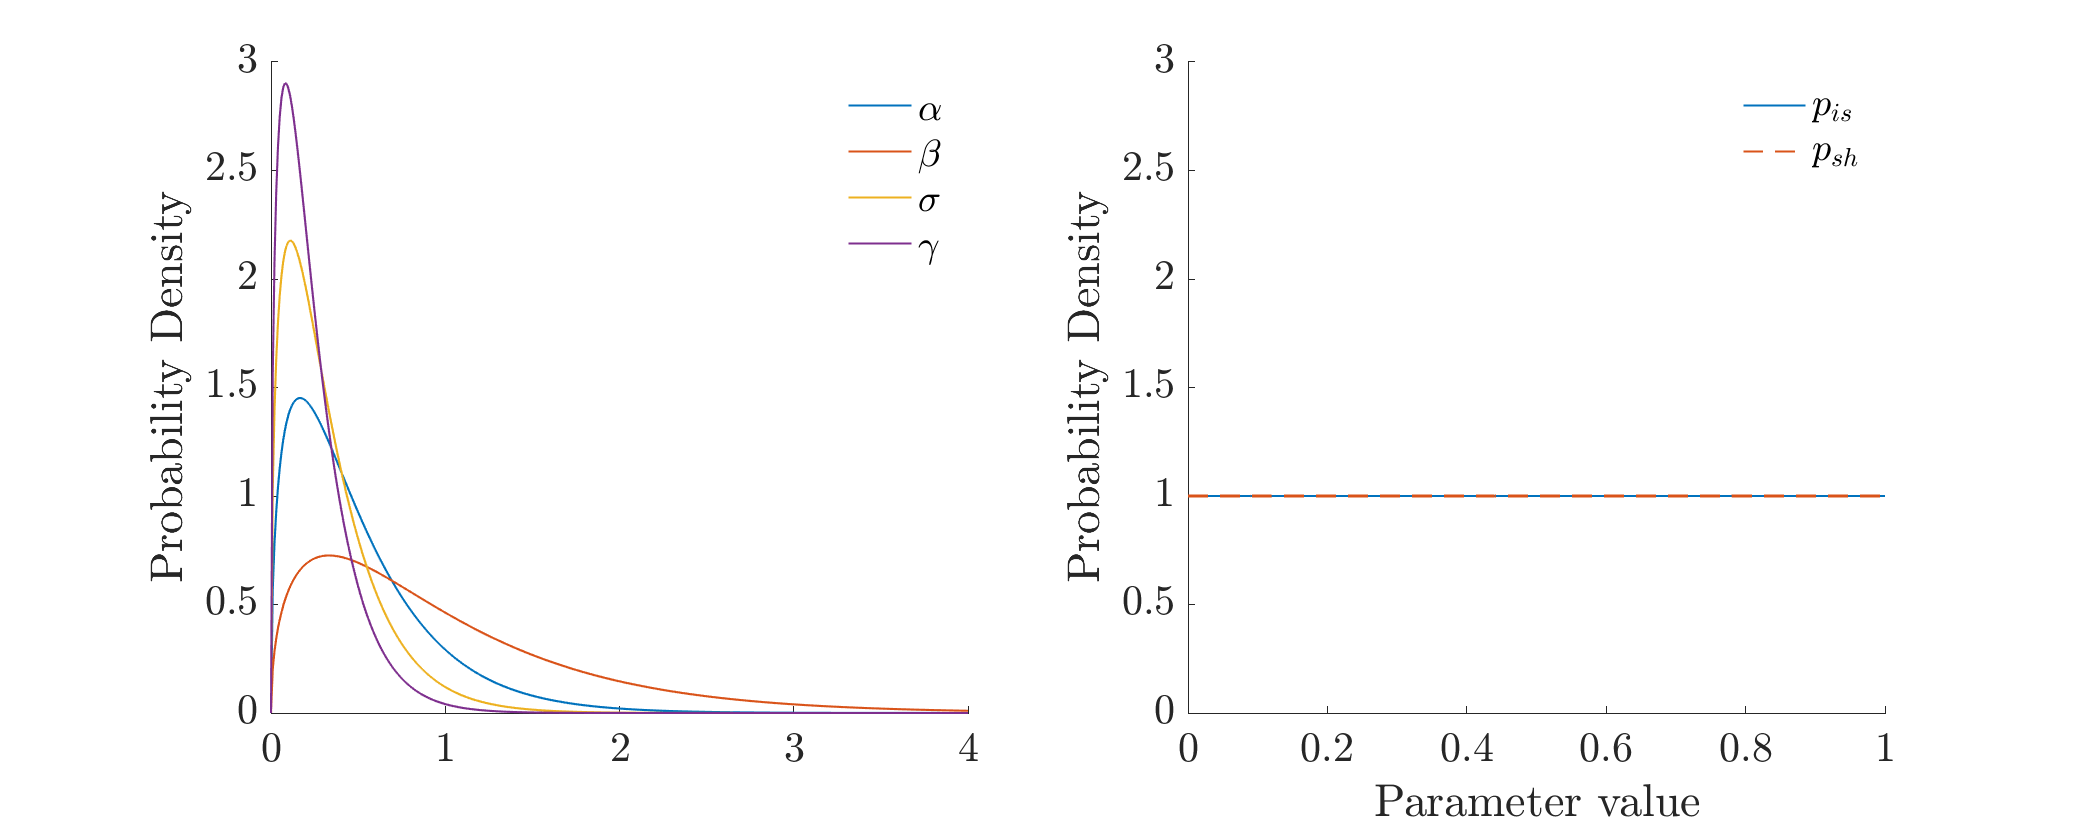
\includegraphics[scale=0.4]{Figs/priors}
	%		\vspace{-10mm}
	\caption{Gamma distributions (left) were used as priors for parameters $\alpha$, $\beta$, $\sigma$, and $\gamma$, while uniform distributions (right) defined on the support $(0,1)$ were used for $p_{is}$ and $p_{sh}$.}
	\label{fig:priors}
\end{figure}


\subsubsection{Implementation of Metropolis-Hastings Algorithm}
The log-likelihood and log-prior defined above are then combined to form the log-posterior,
\begin{align} \notag
\ln P(\alpha, \beta, \gamma, \sigma, p_{is}, p_{ih} | FT, FC, C) \propto &\ln P(FT, FC, C | \alpha, \beta, \gamma, \sigma, p_{is}, p_{ih} ) \\ 
&+ \ln P(\alpha, \beta, \gamma, \sigma, p_{is}, p_{ih})
\end{align}
As it is not feasible to sample directly from this log-posterior, the Metropolis-Hastings (MH) algorithm is used. The general MH algorithm described in Chapter \ref{chp: Lit Review}, Section \ref{sec: MCMC} must first be modified to work on the log-scale. This is set out in Algorithm \ref{alg: log Metropolis-Hastings}. The main differences here compared to the general MH algorithm described in Algorithm \ref{alg: Metropolis-Hastings General} is the form of the acceptance probability and the choice of proposal distribution.\\
Following the discussion on choosing an appropriate proposal distribution in Subsection \ref{subsec: proposal}, for transmission parameters $\alpha, \beta, \sigma, \gamma > 0$ new samples are drawn from a log-normal distribution. Let $g(x) = \exp(x)$, so that $g^{-1}(x) = \ln(x)$ and the Jacobian is $\frac{d}{dx}g^{-1}(x) = \frac{1}{x}$.
For the probability parameters $p_{is}, p_{sh} \in (0,1)$, new samples can be drawn from the so called `logit-normal' distribution. Here, let $g(x) = \frac{\exp(x)}{\exp(x)+1}$, then $g^{-1}(x) = \ln(x) - \ln(1-x)$ and the Jacobian is $\frac{d}{dx}g^{-1}(x) = \frac{1}{x(1-x)}$. \\
This process is demonstrated in Figure \ref{fig:transformed proposal}. For a current sample $x_1$ (blue spot) of a random variable $X_1>0$ in plot (a), a new sample $x_1'$ (red spot) is drawn from a log-normal distribution ($x_1' \sim$ Lognormal$(\ln x_1, \sigma)$, for a chosen $\sigma$) by taking the logarithm of $x_1$ and proposing $\ln x_1'$ using a symmetric proposal distribution (b). The logarithm of the new sample $\ln x_1'$ is then transformed back to $x_1'$ on the original space (a). Plots (c) and (d) show the same procedure for another random variable $X_2 \in [0,1]$ using the logit-normal proposal. \\
Using the change of variables, the proposal distribution can be expressed in terms of the normal distribution and the Jacobian, i.e. $Q(x|x')=f_{\mathcal{N}}(x | x')J(x)$. Then in general the logarithm of the acceptance probability can be expressed
\begin{align} \notag
	\ln p_{acc} &= \ln \frac{P(x') f(x | x') J(x)}{P(x)f(x'|x)J(x')} \\ \notag
	&= \ln \frac{P(x')J(x)}{P(x)J(x')} & \text{since } f_\mathcal{N}(x | x') = f_\mathcal{N}(x' | x)\\
	&= \ln P(x')+\ln J(x) - \ln P(x) - \ln J(x')
\end{align}
Finally, as it was assumed that all of the target parameters are independent, the proposal of a given sample is the product of individual proposals. It follows that the Jacobian of a given sample is the product of individual Jacobians, that is $J(x) = J(\alpha)J(\beta)J(\sigma)J(\gamma)J(p_{is})J(p_{sh})$. On the log scale this becomes the sum of logs \[ \ln J(x)  = \ln J(\alpha) + \ln J(\beta) + \ln J(\sigma) + \ln J(\gamma) + \ln J(p_{is}) + \ln J(p_{sh}) \]
For a current sample $x=(a,b,s,j,i,h)$ and proposal sample $x'=(a',b',s',j',i',h')$, the log-acceptance probability is
\begin{align} \notag
\ln p_{acc} &= \ln P(\alpha=a, \beta=b, \gamma=j, \sigma=s, p_{is}=i, p_{ih}=h | FT, FC, C) \\ \notag
&+ \ln J(a) + \ln J(b) + \ln J(s) + \ln J(j) + \ln J(i) + \ln J(h) \\ \notag
&- \ln P(\alpha=a', \beta=b', \gamma=j', \sigma=s', p_{is}=i', p_{ih}=h' | FT, FC, C) \\
&- \ln J(a') + \ln J(b') + \ln J(s') + \ln J(j') + \ln J(i') + \ln J(h') 
\end{align}

\begin{algorithm}[H]
	\SetAlgoLined
	%	\KwResult{Write here the result }
	Set initial guess $X(0) = x_0$ \;
	Choose a proposal distribution $Q(x'|x)$ to generate new samples $x'$ given the current sample $x$\;
	\For{$i=1:N$}{
		Let $x = X(i-1)$ \;
		Draw a new sample $x'$ from $Q(x'|x)$ \;
		Compute the log-acceptance probability $\ln p_{acc} = \min\{ 0, \ln P(x') - \ln P(x) + \ln Q(x'|x) - \ln Q(x|x')\}$ \;
		Draw another random number $u \sim \text{Uniform}(0,1)$ \;
		\eIf{$\log u < \ln p_{acc}$}{
			Accept $x'$, set $X(i) = x'$ \;
		}{
			Reject $x'$, set $X(i) = x$ \;
		}
	}
	\caption{Metropolis-Hastings Algorithm (Log-Scale)}
	\label{alg: log Metropolis-Hastings}
\end{algorithm}

